%%%%%%%%%%%%%%%%%%%%%%%%%%%%%%%%%%%%%%%%%%%%%%%%%%%%%%%%%%%%%%%%%%%%%%%
% Created on Mon June 5, 2023
% @author: Giselle Labrador Badia (@gisslab)
% Last modified: Friday Sept 22, 2023 

% Description:
%
% This report analyses OB auction files for the early Covid period. 
% It is based on the code files auction_prices_analysis.py, 
% auction_prices_timeseries_plots, fed_mbs
%%%%%%%%%%%%%%%%%%%%%%%%%%%%%%%%%%%%%%%%%%%%%%%%%%%%%%%%%%%%%%%%%%%%%%%




\documentclass[11pt,a4paper]{article}


\usepackage[utf8]{inputenc}
\usepackage[spanish,english]{babel}
\usepackage{apacite}
\usepackage[round]{natbib}
\usepackage{hyperref}
\bibliographystyle{apacite}


\usepackage[margin = 1in, top=1.5cm,bottom=1.5cm]{geometry}% Margins
\setlength{\parindent}{2em}
\setlength{\parskip}{0.3em}
\usepackage{setspace} % Setting the spacing between lines
\usepackage{hyperref} % To create hyperlinks within the document
\spacing{1.15}

%images
\usepackage{graphicx}
% \usepackage{subcaption}
\usepackage{caption}
% subcaption was interfering with the figure count, fix below
\usepackage{subcaption, xparse}

% to read mid rule
\usepackage{booktabs}

\usepackage[capposition=top]{floatrow}
\captionsetup[sub]{font=footnotesize,labelfont={bf,sf}}

\begin{document}

\title{QE and the Mortgage Market during the COVID-19 Pandemic}

\maketitle



\section{FED purchases of MBS}

The following figures show the daily time series of amounts and prices of FED purchases of MBAs for Fannie Mae and Freddie Mac
 products and 30-year maturity in the early COVID period. We plot by month the total amount by coupon and the mean price. If it only shows a dot is because there is only one month of data for that coupon. The period is January 2020 to April 2021. The prices and quantities are aggregated monthly by trade date. 


\begin{figure}[h]
    \centering
    \begin{subfigure}[b]{0.49\textwidth}
      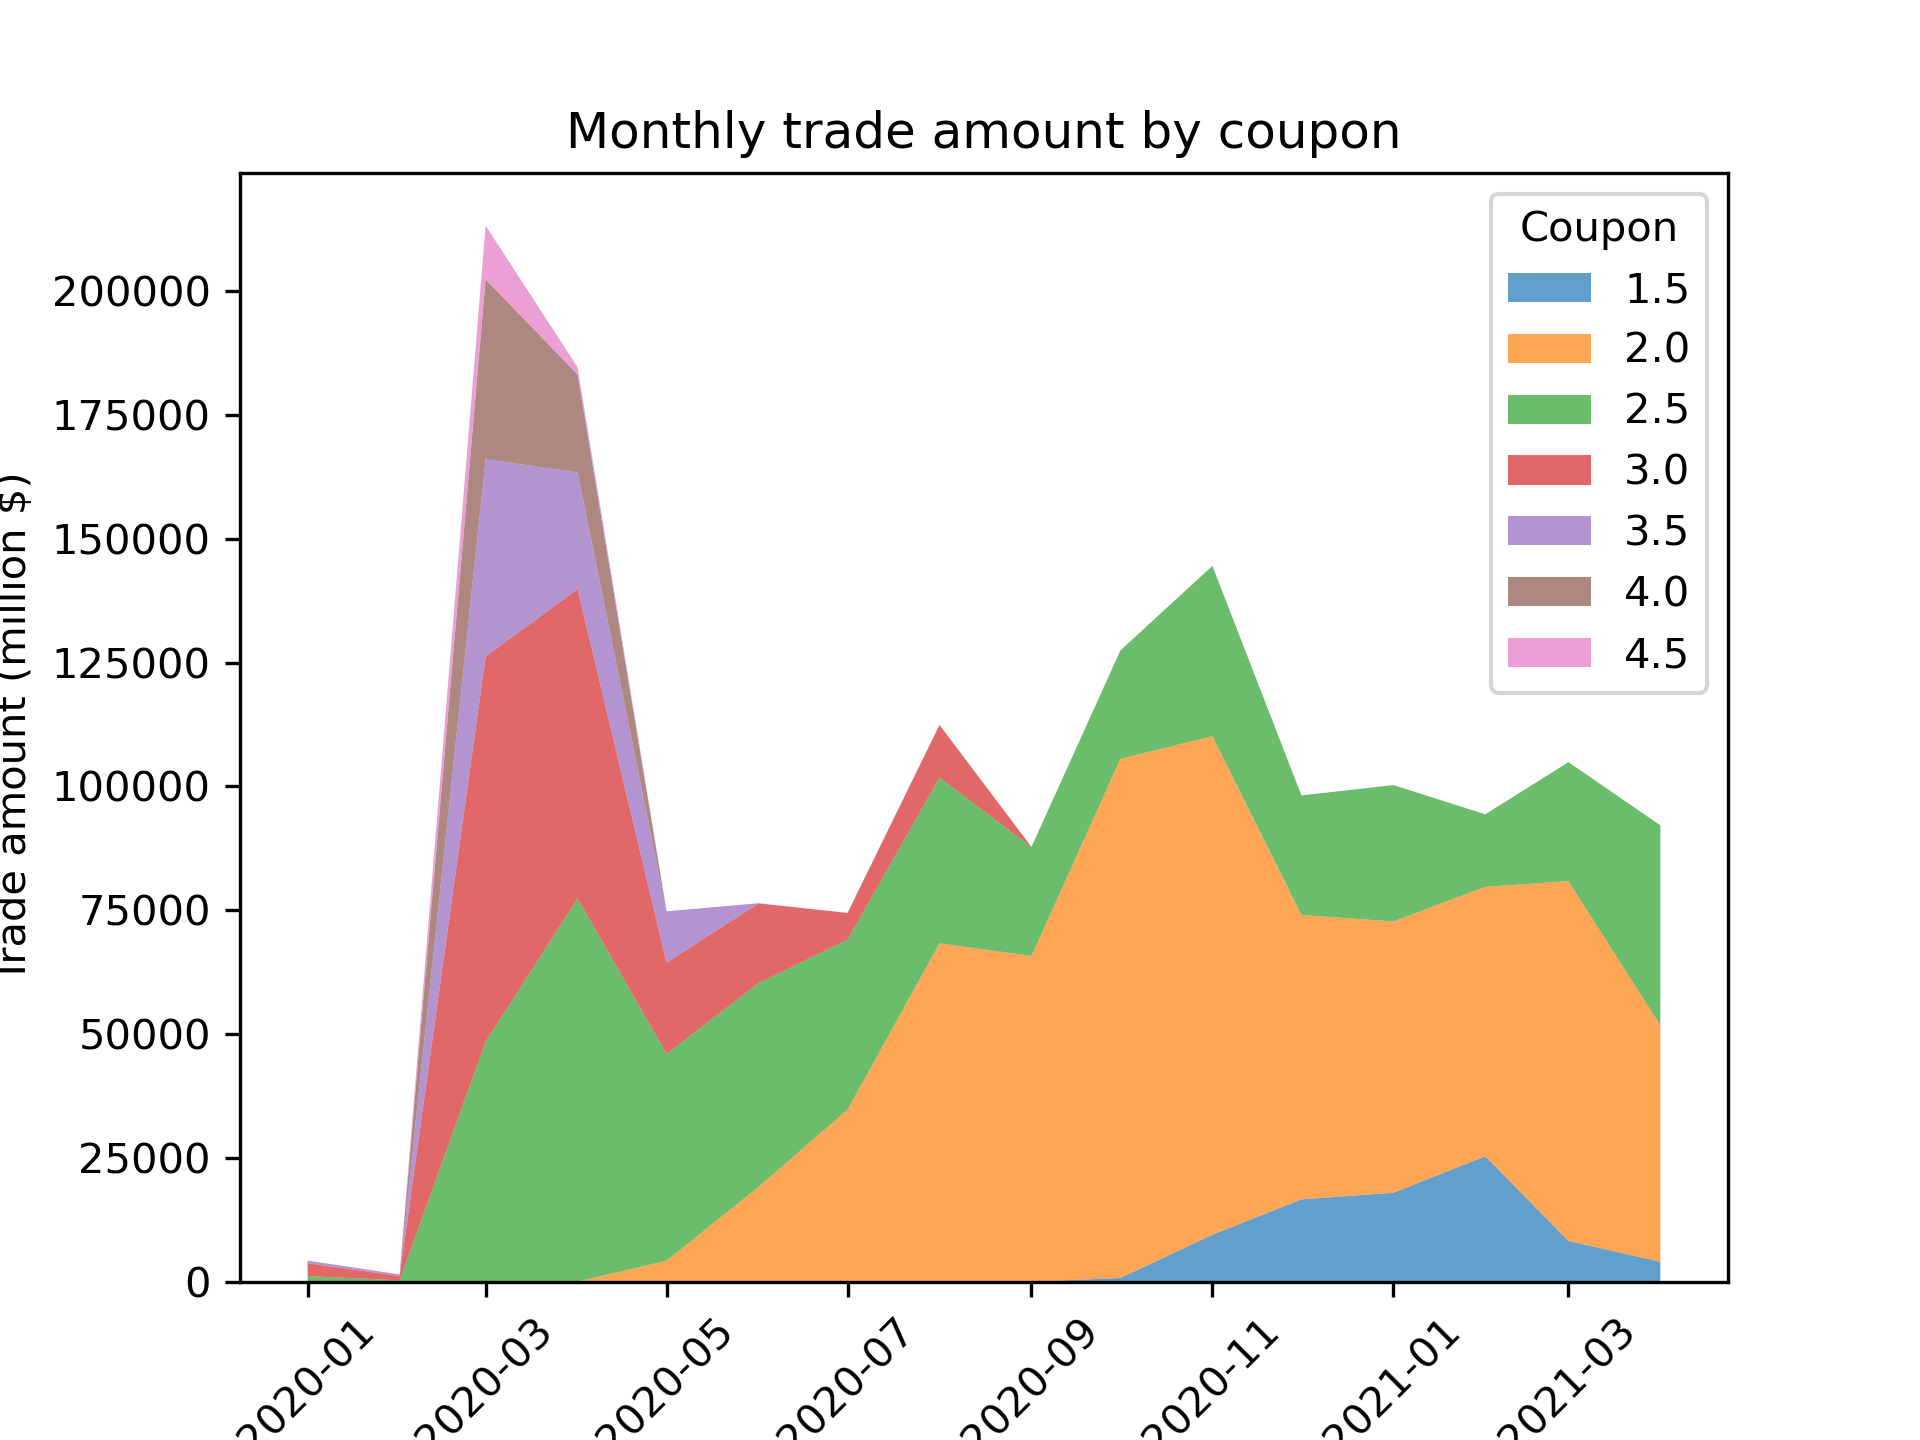
\includegraphics[width=0.998\textwidth]{../results/figures/fed_monthly_trade_amount_by_coupon.png}
      \caption{ Quantity by trade date}
     \end{subfigure}
     \begin{subfigure}[b]{0.49\textwidth}
      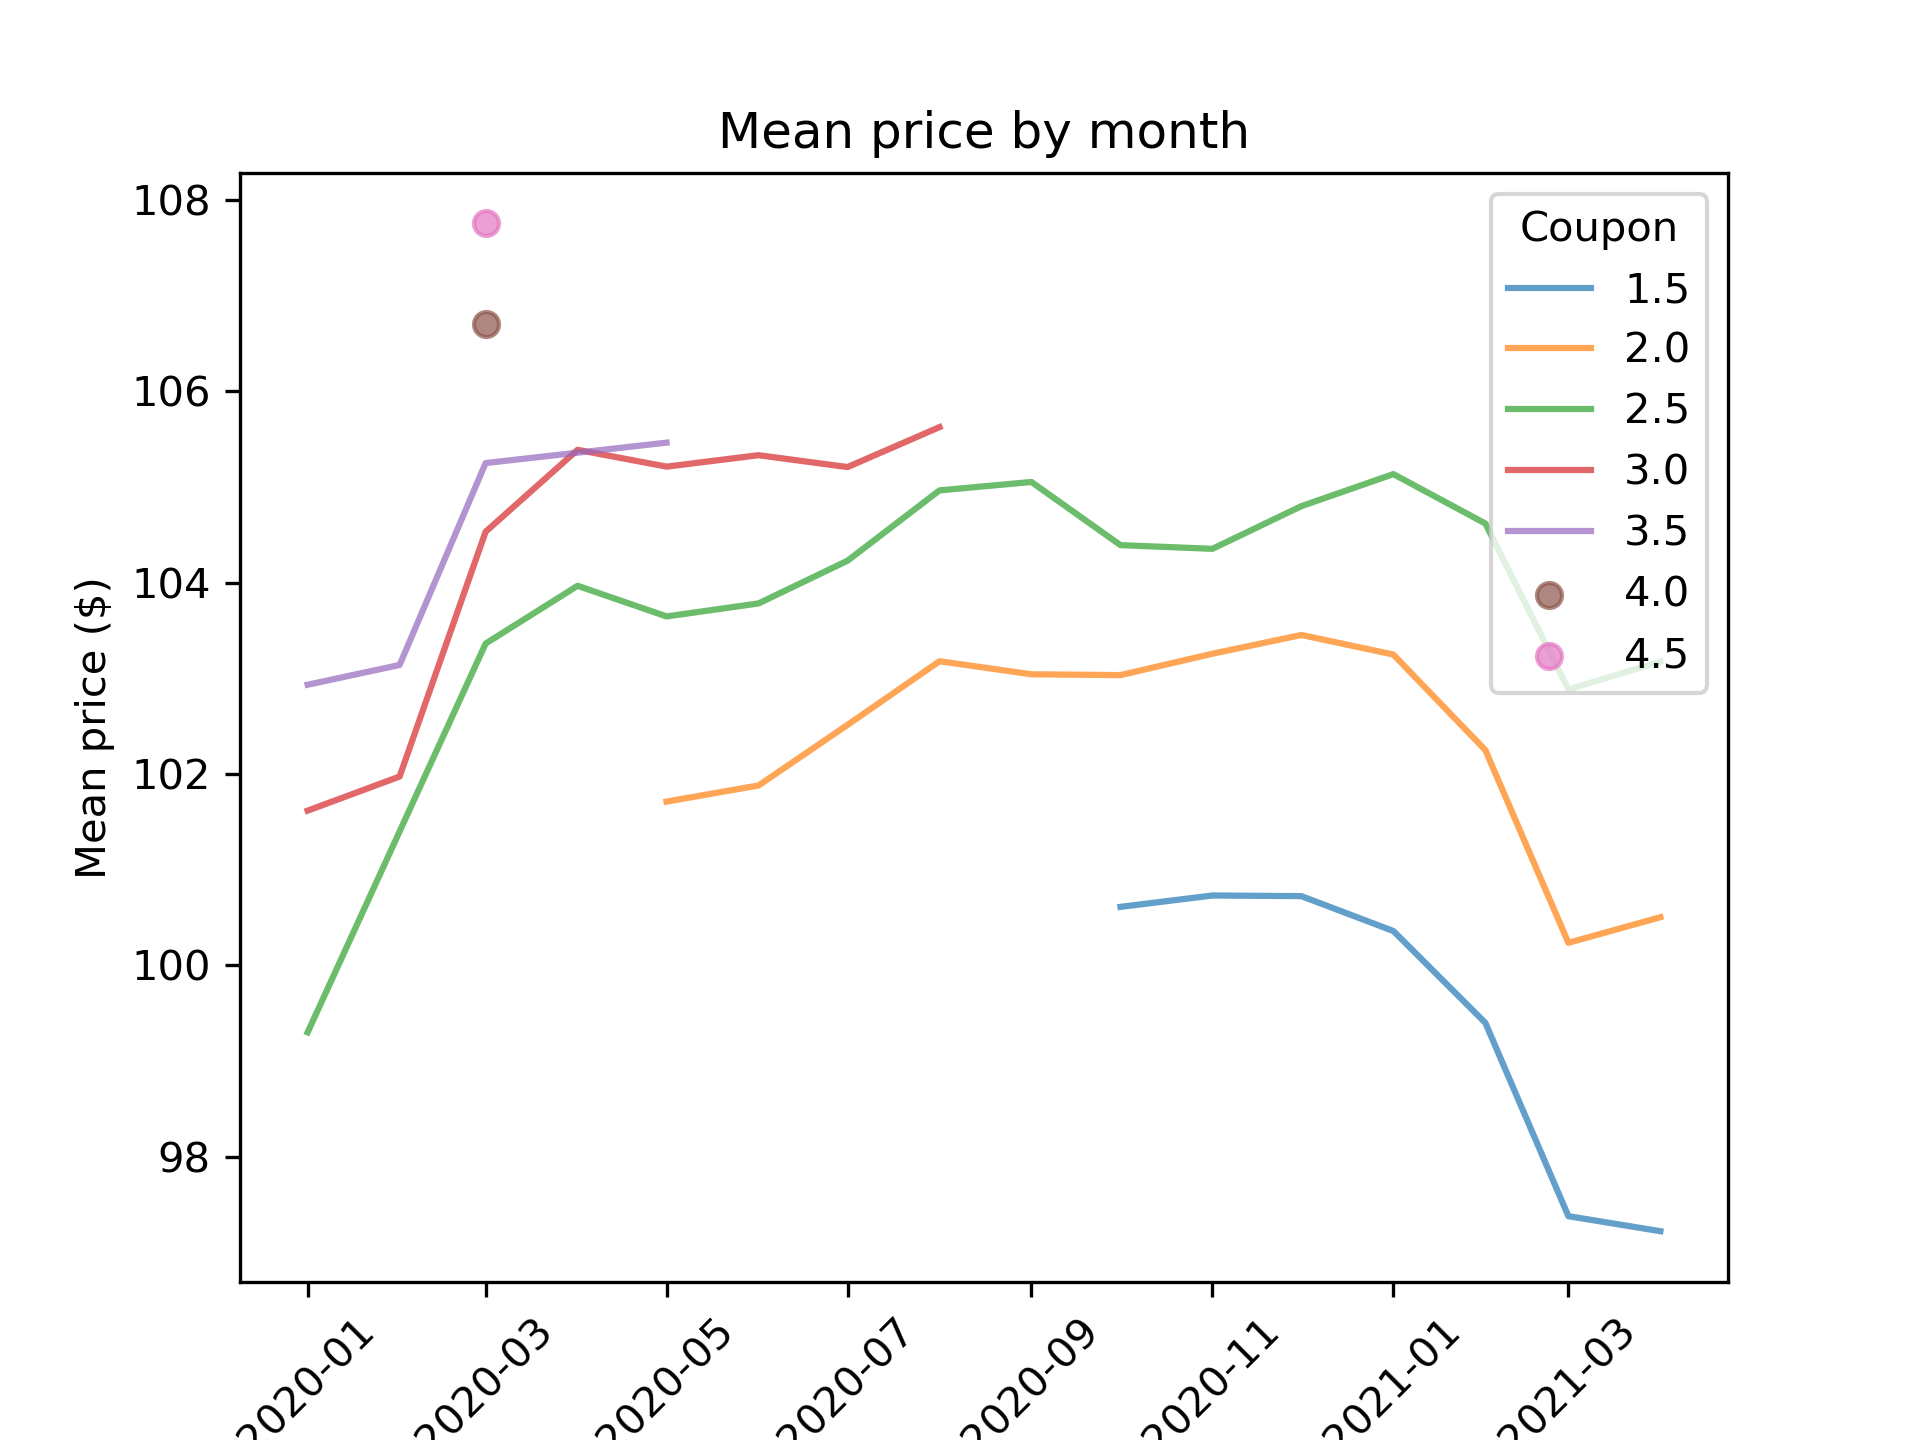
\includegraphics[width=0.998\textwidth]{../results/figures/fed_monthly_price_mean_by_coupon.png}
      \caption{ Price by trade date}
     \end{subfigure}
     \caption{FED purchases of Fannie Mae and Freddie Mac MBS securities  in the early COVID period} 
     \begin{minipage}{\textwidth}
      \footnotesize{\textit{Notes:} The figure shows the monthly time series of trade amounts and prices of FED purchases of Fanny Mae and Fredy Mac products and 30-year maturity. Colors represent different coupons. } 
        \end{minipage}
\end{figure}

\pagebreak

Now, we choose coupon 2.5 which was traded in the majority of periods, and plot the daily time series prices of FED purchases of the same product. Panel (c) shows the daily time series of prices normalized by the Bloomberg TBA price.  The net price is then calculated as the difference between the FED price and the TBA price. This is only for FED purchases that we categorized as one-month forward\footnote{$x$ months forward is defined as when the trade date is between $x$ months and $x+1$ month before the settlement date.} One month forward was chosen since it is the most common forward period for FED purchases. 

\begin{figure}[h]
  \centering
  \begin{subfigure}[b]{0.49\textwidth}
    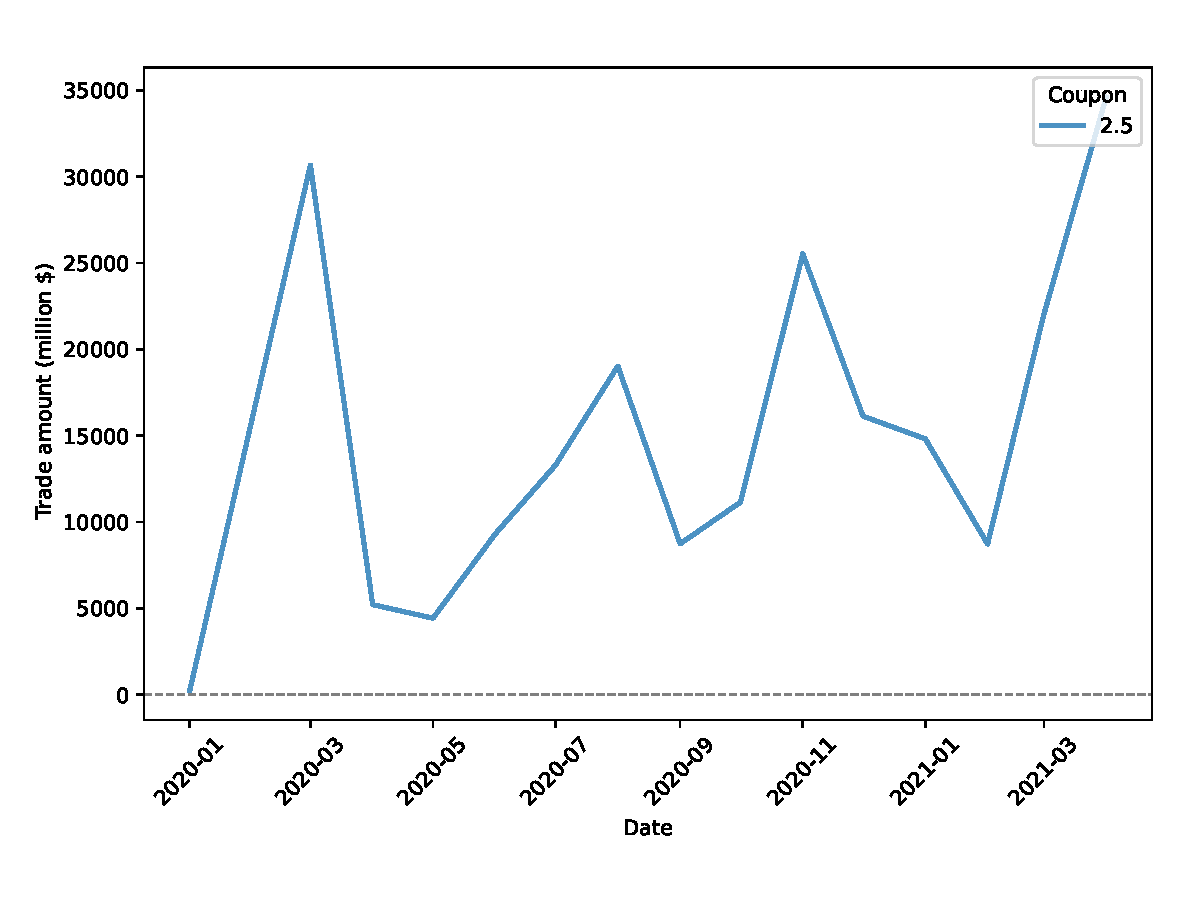
\includegraphics[width=0.998\textwidth]{../results/figures/fed_trade_amount_mat30_loan1_timeseries_cpmonthly_coup2.5}
    \caption{ Quantity }
    \end{subfigure}
  \begin{subfigure}[b]{0.49\textwidth}
    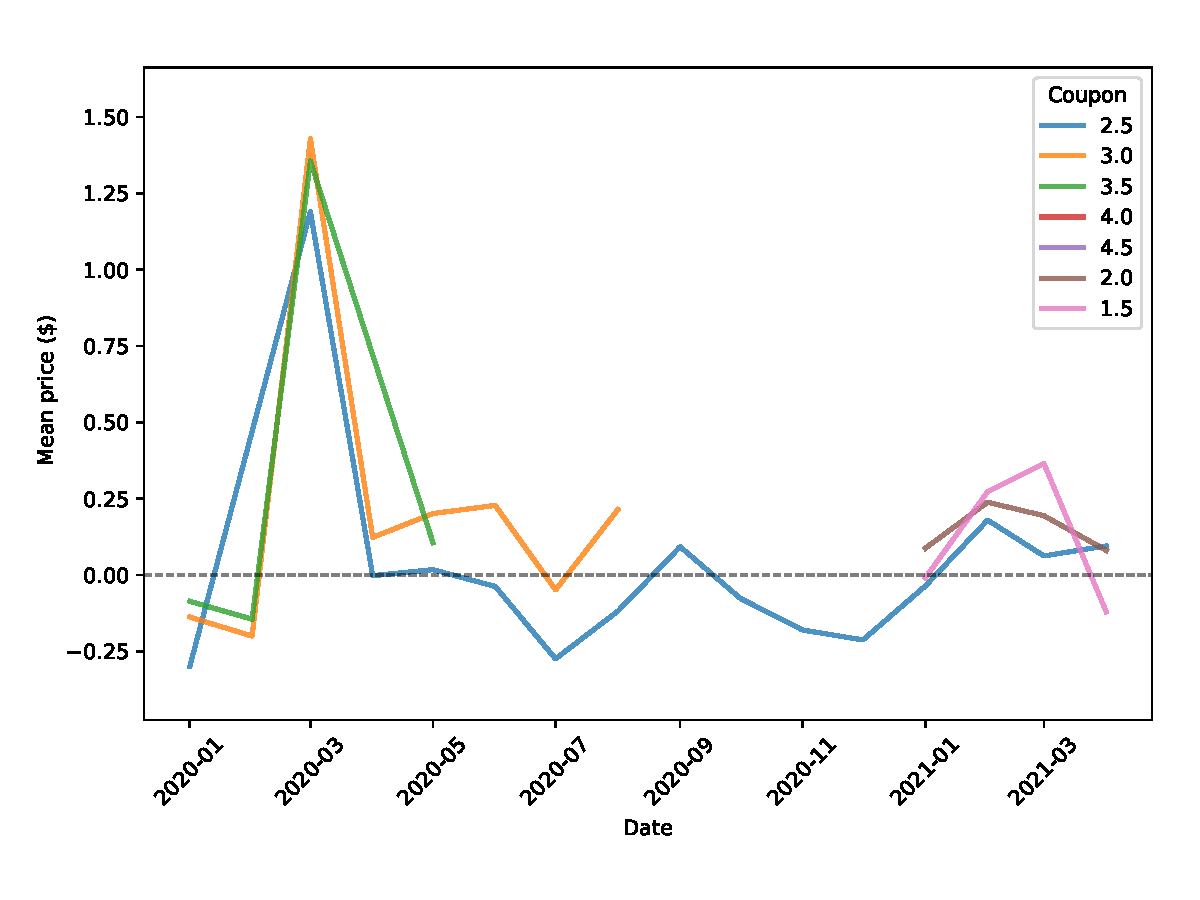
\includegraphics[width=0.998\textwidth]{../results/figures/fed_price_mean_mat30_loan1_timeseries_cpmonthly_coup2.5}
    \caption{ Price }
   \end{subfigure}
   \begin{subfigure}[b]{0.49\textwidth}
    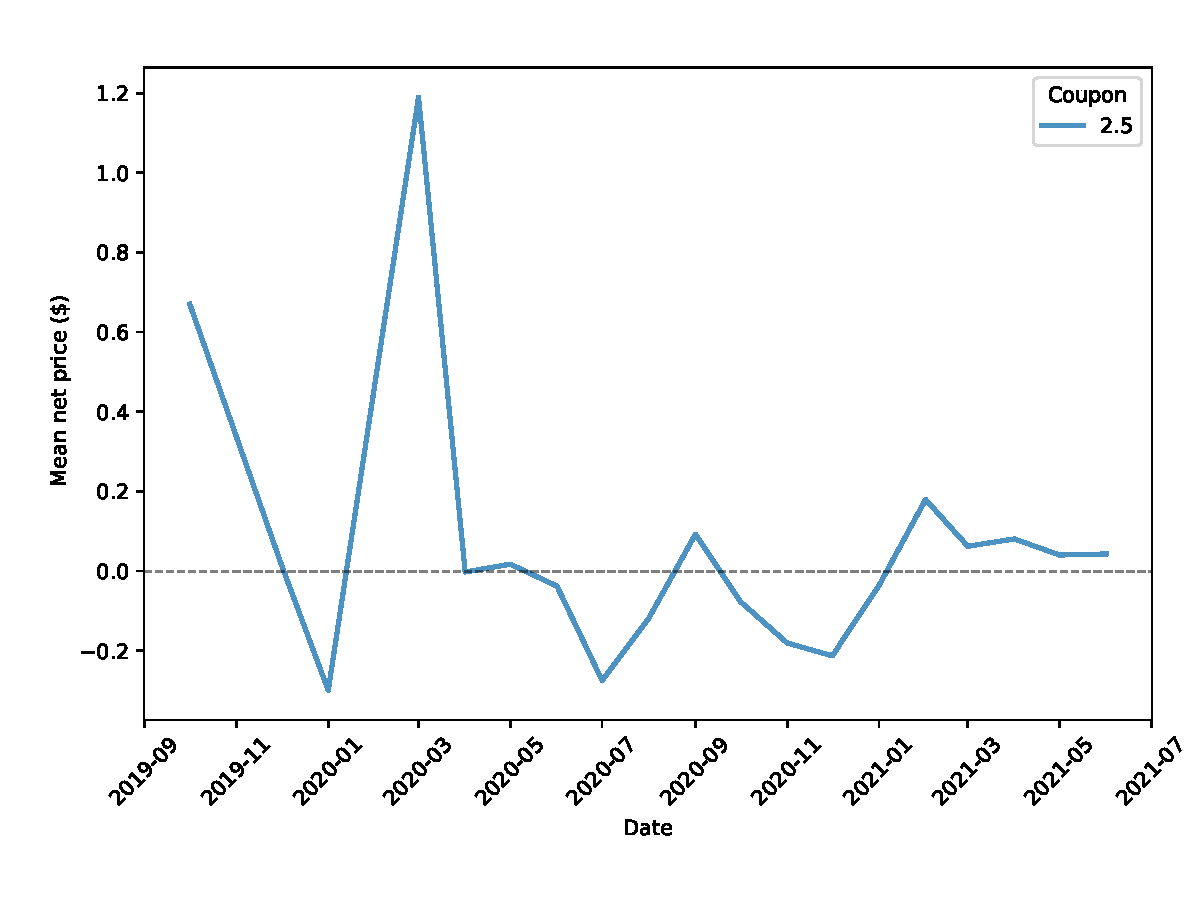
\includegraphics[width=0.998\textwidth]{../results/figures/fed_price_mean_mat30_loan1_timeseries_cpmonthly_normalized_coup2.5}
    \caption{ Net price}
   \end{subfigure}
   \begin{subfigure}[b]{0.49\textwidth}
    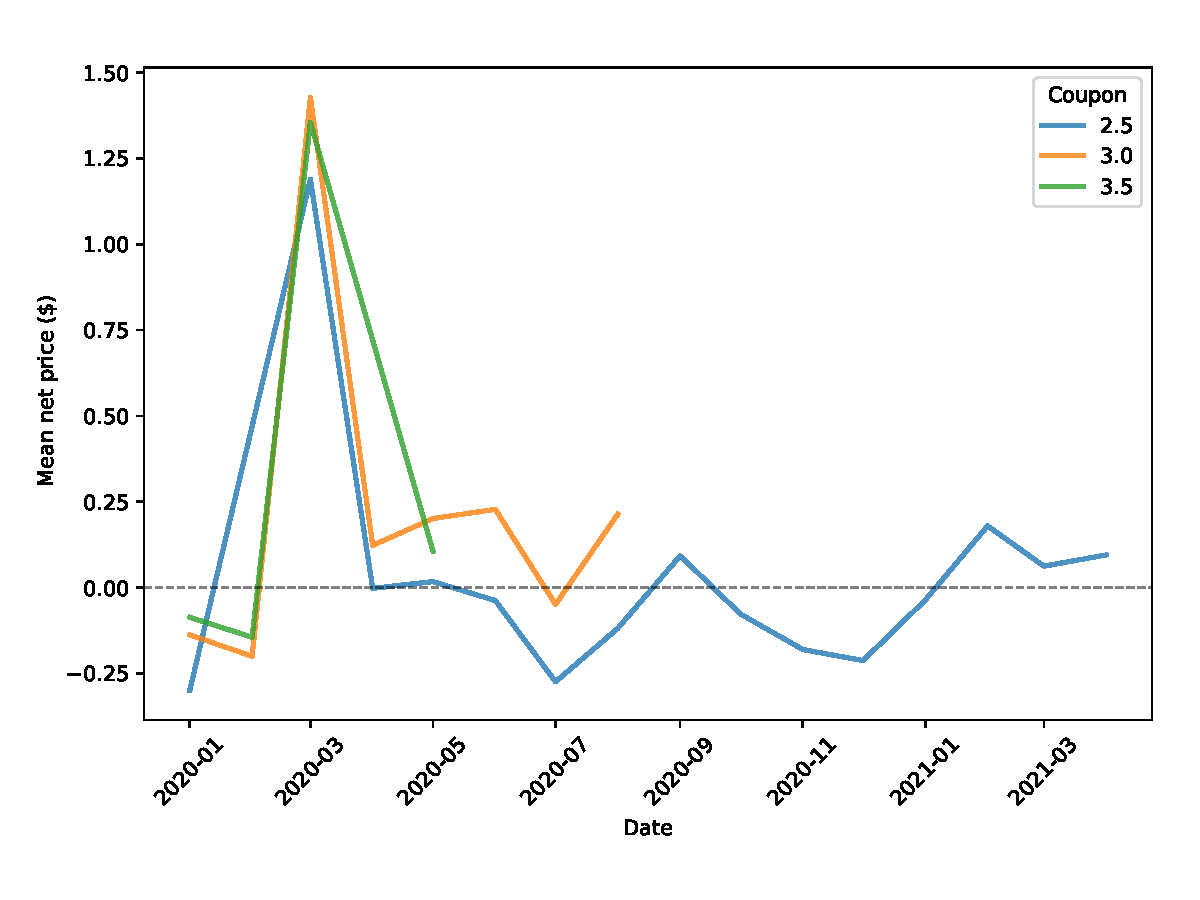
\includegraphics[width=0.998\textwidth]{../results/figures/fed_price_mean_mat30_loan1_timeseries_cpmonthly_normalized}
    \caption{ Comparison of coupons net price }
   \end{subfigure}
   \caption{FED purchases of Fannie Mae and Freddie Mac MBS securities  in the early COVID period} 
   \begin{minipage}{\textwidth}
      \footnotesize{\textit{Notes:} The figure shows the monthly time series of trade amounts and prices of FED purchases of Fanny Mae and Fredy Mac products and 30-year maturity. Colors represent different coupons. } 
      \end{minipage}
\end{figure}


\pagebreak
\section{OB Auctions in the Early Covid Period}


The following figure shows a histogram of all bids for all auctions in the OB platform between January 2020 and December 2021. 
The product is Conforming loans with a 30-year maturity. 


%figure 

\begin{figure}[h]
    \centering
    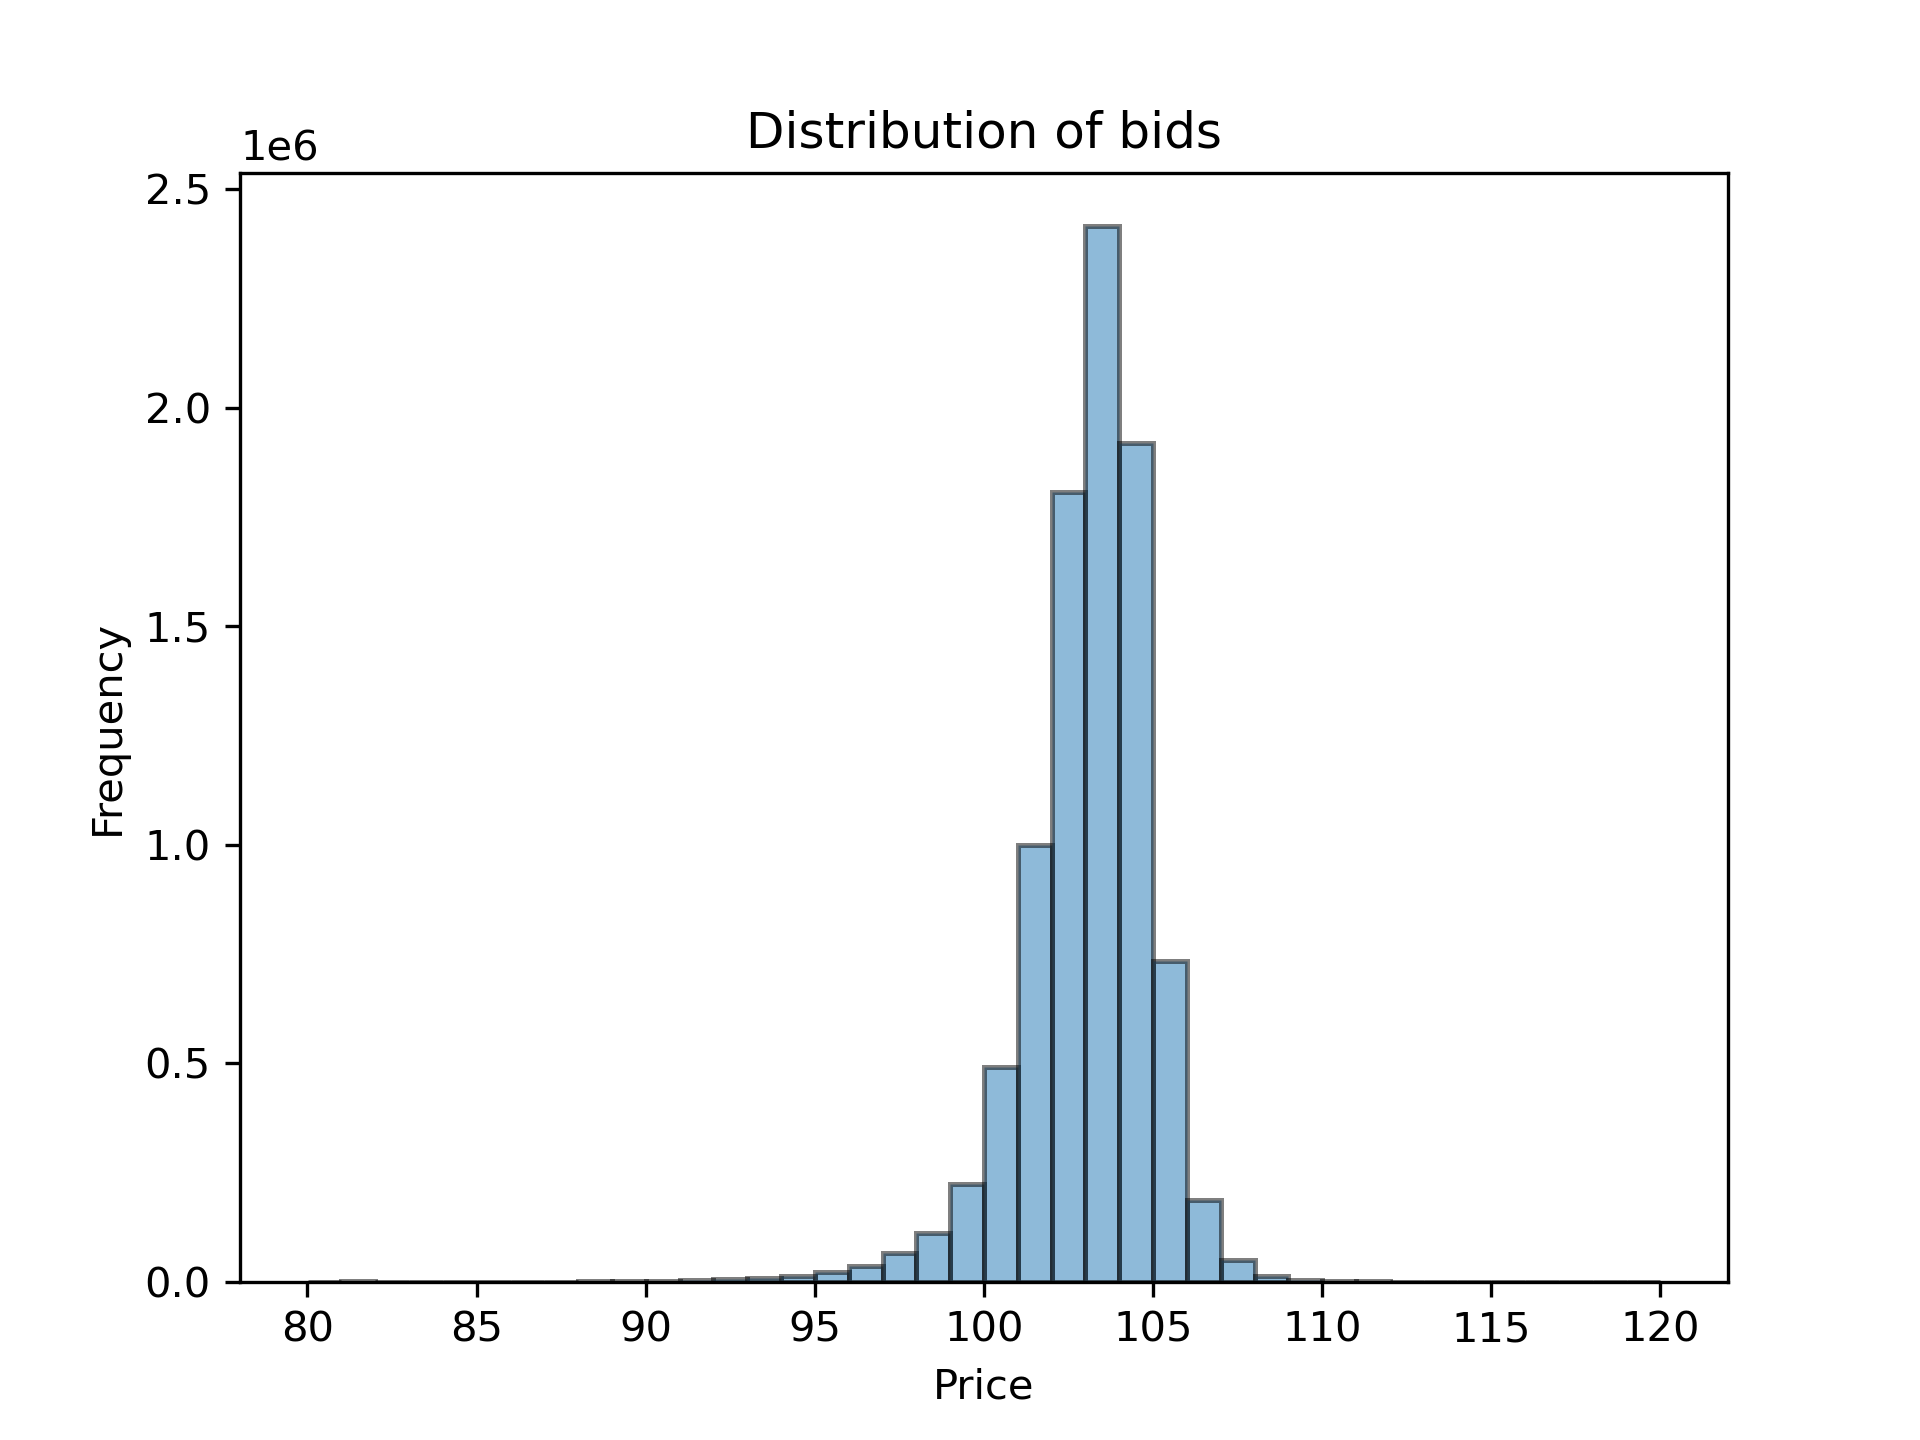
\includegraphics[width=0.62\textwidth]{../results/figures/distribution_of_bids.png}
    \caption{Histogram of all bids for all auctions in the oB platform for January, February, March, and April 2020. The product is Conforming loans with a 30-year maturity.}
    \begin{minipage}{\textwidth}
        \footnotesize{\textit{Notes:} The figure shows a histogram of all bids for all auctions in the OB platform for January, February, March, and April 2020. The product is Conforming loans with a 30-year maturity. } 
        \end{minipage}
\end{figure}

This figure shows a histogram of the note rates by auction for the same period and product.
\begin{figure}[h]
  \centering
  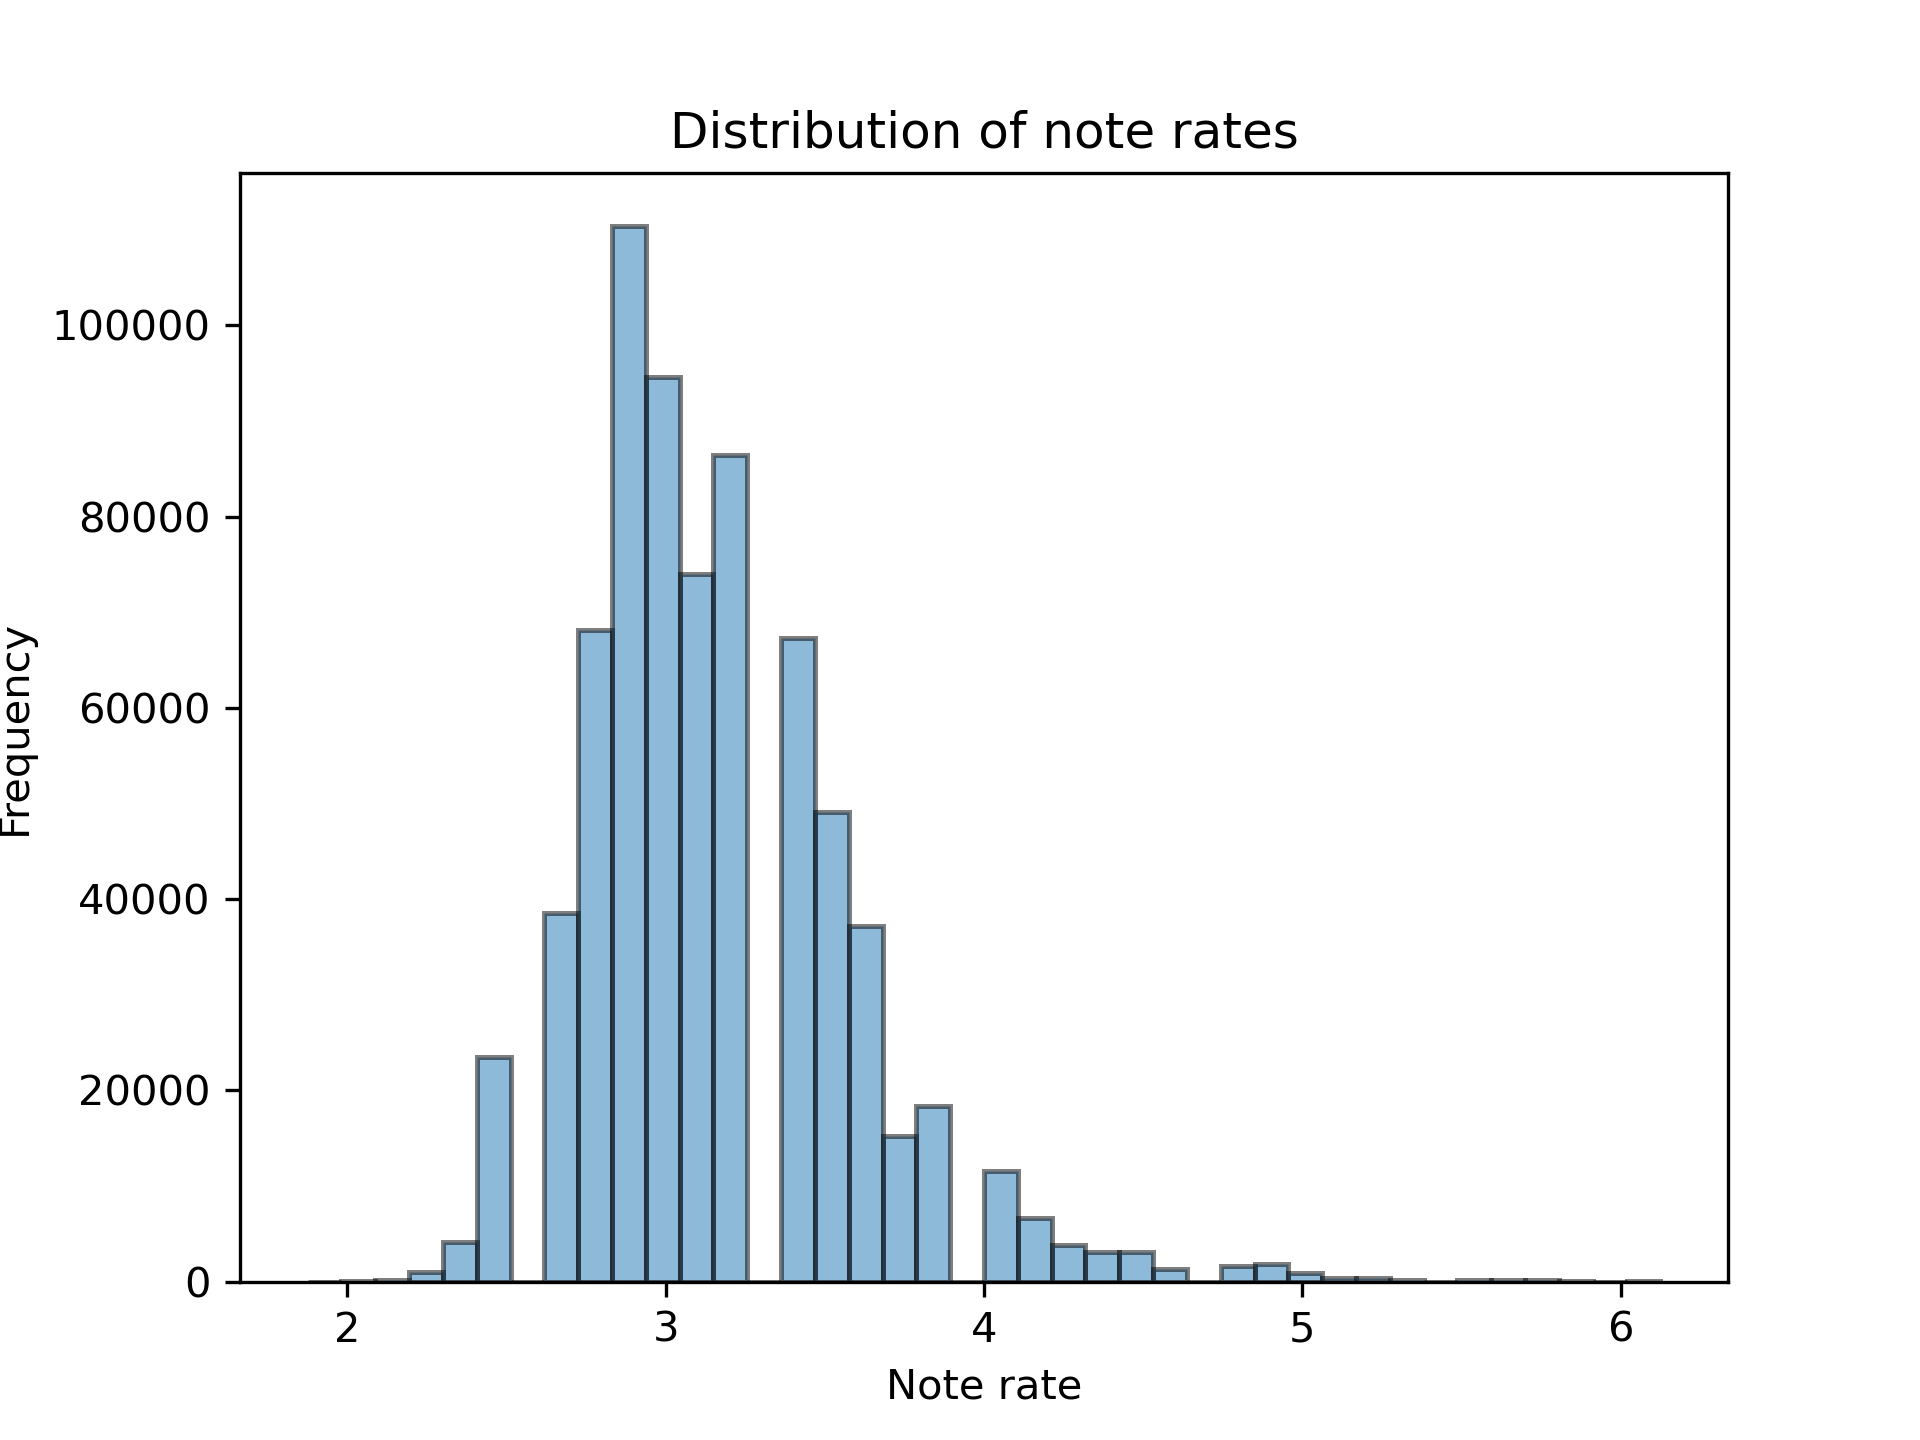
\includegraphics[width=0.62\textwidth]{../results/figures/distribution_of_noterates.png}
  \caption{Histogram of all bids for all auctions in the oB platform for January, February, March, and April 2020. The product is Conforming loans with a 30-year maturity.}
  \begin{minipage}{\textwidth}
      \footnotesize{\textit{Notes:} The figure shows a histogram of all note rates of auctioned loans in the OB platform for the months of January, February, March, and April 2020. The product is Conforming loans with a 30-year maturity. } 
      \end{minipage}
\end{figure}


\pagebreak
Table 1 shows descriptive statistics for important outcomes at the auction level for the same period and product. 

%table

\begin{table}[h]
    \centering
    \begin{tabular}{lrrrrrrrr}
\toprule
{} &    count &    mean &     std &     min &     25\% &  median &     75\% &      max \\
\midrule
Loan amount            &  80848.0 &  274.37 &  126.61 &   23.25 &  179.74 &  257.00 &  354.33 &  1470.00 \\
Note rate              &  80848.0 &    3.71 &    0.45 &    2.25 &    3.38 &    3.62 &    3.88 &     6.12 \\
Price                  &  80848.0 &  104.04 &    1.36 &   94.03 &  103.25 &  104.02 &  104.82 &   120.00 \\
Days to auction        &  80704.0 &    4.76 &    7.96 & -326.00 &    1.00 &    3.00 &    6.00 &   288.00 \\
Number of participants &  80848.0 &   11.35 &    5.52 &    1.00 &    8.00 &   12.00 &   15.00 &    32.00 \\
Number of bulk bidders &  80848.0 &    7.37 &    6.08 &    0.00 &    0.00 &    8.00 &   12.00 &    27.00 \\
Sell rate              &  80848.0 &    0.77 &    0.42 &    0.00 &    1.00 &    1.00 &    1.00 &     1.00 \\
Rate sell to winner    &  80848.0 &    0.49 &    0.50 &    0.00 &    0.00 &    0.00 &    1.00 &     1.00 \\
\bottomrule
\end{tabular}

    \caption{Descriptive statistics at the auction level. }
    \begin{minipage}{\textwidth}
        \footnotesize{\textit{Notes:} The table shows descriptive statistics at the auction level of observation for the months of January, February, March, and April 2020. The product is Conforming loans with a 30-year maturity. } 
        \end{minipage}
\end{table}

% \pagebreak

\subsection{Naive comparison before after COVID}

A similar table is depicted for the months of January and February and for the months of March and April. The idea is to compare the outcomes before and after COVID (tables 2 and 3 respectively).

%table
\begin{table}[h]
  \centering
  \begin{tabular}{lrrrrr}
\toprule
{} &    count &    mean &     std &     min &      max \\
\midrule
Loan amount            &  28572.0 &  261.97 &  126.40 &   23.25 &  1184.92 \\
Note rate              &  28572.0 &    3.98 &    0.40 &    2.75 &     6.12 \\
Price                  &  28572.0 &  103.99 &    1.34 &   97.90 &   120.00 \\
Days to auction        &  28517.0 &    5.84 &    8.70 & -326.00 &   288.00 \\
Number of participants &  28572.0 &   12.10 &    5.96 &    1.00 &    32.00 \\
Number of bulk bidders &  28572.0 &    8.82 &    6.45 &    0.00 &    27.00 \\
Sell rate              &  28572.0 &    0.84 &    0.37 &    0.00 &     1.00 \\
Rate sell to winner    &  28572.0 &    0.50 &    0.50 &    0.00 &     1.00 \\
\bottomrule
\end{tabular}

  \caption{Descriptive statistics at the auction level January and February 2020. }
  \begin{minipage}{\textwidth}
      \footnotesize{\textit{Notes:} The table shows descriptive statistics at the auction level of observation for the months of January and  February 2020. The product is Conforming loans with a 30-year maturity. } 
      \end{minipage}
\end{table}

\begin{table}[h]
  \centering
  \begin{tabular}{lrrrrr}
\toprule
{} &    count &    mean &     std &     min &      max \\
\midrule
Loan amount            &  50120.0 &  280.90 &  126.22 &   26.16 &  1470.00 \\
Note rate              &  50120.0 &    3.56 &    0.41 &    2.25 &     6.12 \\
Price                  &  50120.0 &  104.08 &    1.36 &   94.03 &   120.00 \\
Days to auction        &  50068.0 &    4.18 &    7.36 & -244.00 &   234.00 \\
Number of participants &  50120.0 &   10.98 &    5.22 &    1.00 &    30.00 \\
Number of bulk bidders &  50120.0 &    6.60 &    5.73 &    0.00 &    26.00 \\
Sell rate              &  50120.0 &    0.74 &    0.44 &    0.00 &     1.00 \\
Rate sell to winner    &  50120.0 &    0.49 &    0.50 &    0.00 &     1.00 \\
\bottomrule
\end{tabular}

  \caption{Descriptive statistics at the auction level of March and April 2020. }
  \begin{minipage}{\textwidth}
      \footnotesize{\textit{Notes:} The table shows descriptive statistics at the auction level of observation for March and April 2020. The product is Conforming loans with a 30-year maturity. } 
      \end{minipage}
\end{table}

\pagebreak
\section{OB Auctions: Time Series analysis}

This section includes a time series analysis of the OB auctions in the early COVID period. The analysis is done at the monthly level. The product is Conforming loans with a 30-year maturity. It includes the price and quantities of the auctions, as well as the number of auctions per period. Next, distress signs are explored by looking at the number of participants, the number of bids, and the number of bulk bids. Finally, the GSEs' response is by plotting the number of bids by the GSE and the number of auctions won by GSEs.
% In all cases, the analysis includes a comparison between note rates around 3 - 3.75\% and note rates around 4 - 4.75\%.

To analyze the OB auctions, we merge track each loan that was auctioned to know the MBS to which the loan was eventually pooled. Then each loan is matched with an MBS coupon. The matched rate was around 95 \%. Below, we can see the summary of the number of loans per coupon and statistics about the note rates that were pooled in each coupon. 


\begin{table}[h]
  \centering
  \begin{tabular}{rrrrrr}
\toprule
coupon & auctions & \multicolumn{4}{l}{note rate} \\
       &    count &       min &  mean & median &   max \\
\midrule
 1.000 &        5 &     2.000 & 2.000 &  2.000 & 2.000 \\
 1.500 &    42676 &     1.875 & 2.543 &  2.500 & 2.625 \\
 2.000 &   290069 &     2.250 & 2.884 &  2.875 & 3.125 \\
 2.500 &   296294 &     2.750 & 3.287 &  3.250 & 3.625 \\
 3.000 &   141030 &     3.250 & 3.770 &  3.875 & 4.125 \\
 3.500 &    36147 &     3.750 & 4.240 &  4.250 & 4.625 \\
 4.000 &    13199 &     4.250 & 4.687 &  4.750 & 5.125 \\
 4.500 &     5159 &     4.750 & 5.098 &  5.125 & 5.625 \\
 5.000 &     1599 &     5.250 & 5.627 &  5.625 & 6.125 \\
\bottomrule
\end{tabular}

  \caption{Note rate by coupon statistics from January 2020 to December 2021 }
  \begin{minipage}{\textwidth}
      \footnotesize{\textit{Notes:} The table shows descriptive statistics at the auction level of observation for the period January 2020 to December 2021.
     The product is Conforming loans with a 30-year maturity. } 
      \end{minipage}
\end{table}


For this analysis, we define net bid as the difference between the auctions in OB and the TBA Bloomberg price on the day of the auction. Hence, the collapsed OB auction bids are merged by coupon with the TBA Bloomberg price. We focus on conforming loans with a 30-year maturity with 2 months forward. Specially for 2.5 and 3.0 there is a steep decline in the mean note rate pool in the coupons. 

To take a closer look to how the note rates were distributed by coupon, we plot the minimum, maximimum, and mean note rates by coupon over time. 

\begin{figure}[h]
  \centering
  \begin{subfigure}[b]{0.49\textwidth}
      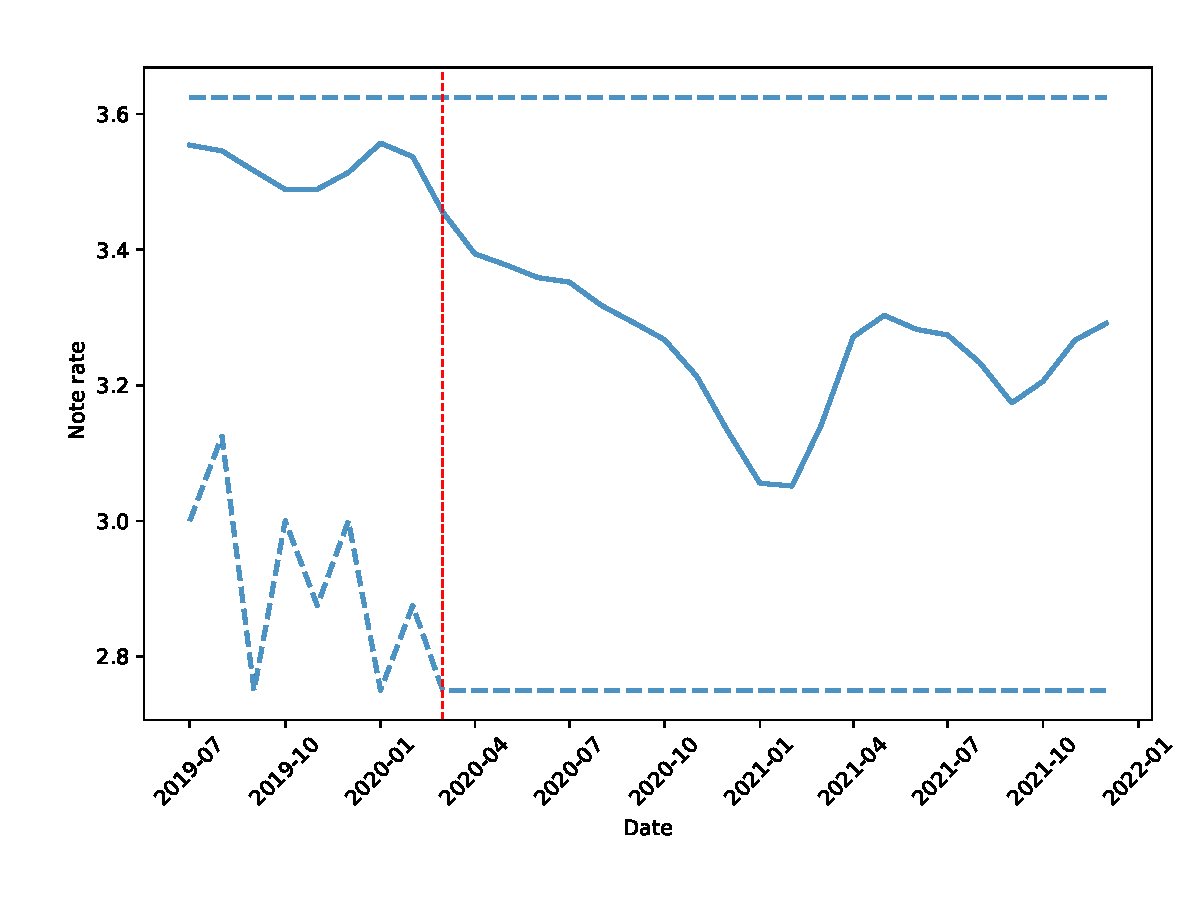
\includegraphics[width=0.998\textwidth]{../results/figures/NoteRate_mean_mat30_loan1_timeseries_nrmonthly_2.5_4_c25.0.pdf}
      \caption{ Coupon 2.5}
     \end{subfigure}
      \begin{subfigure}[b]{0.49\textwidth}
        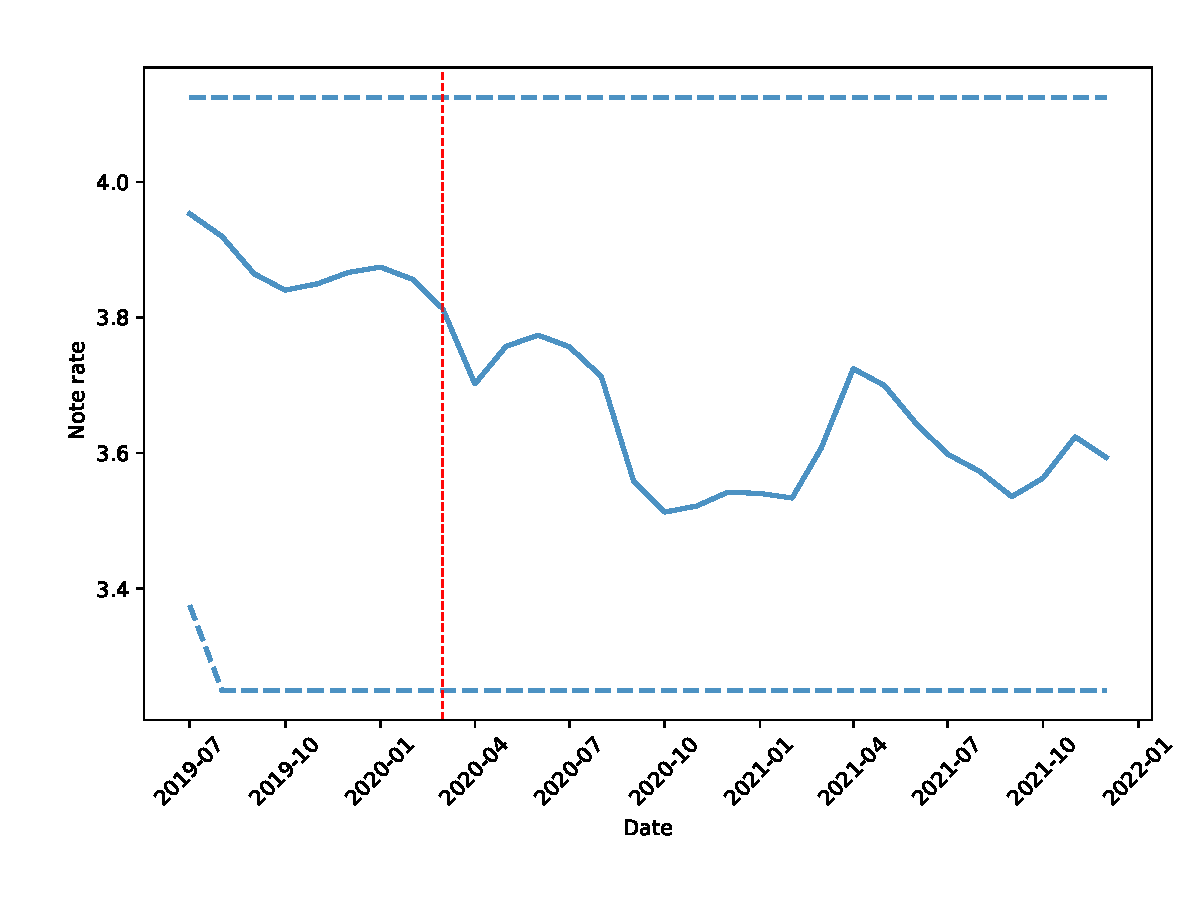
\includegraphics[width=0.998\textwidth]{../results/figures/NoteRate_mean_mat30_loan1_timeseries_nrmonthly_2.5_4_c30.0.pdf}
        \caption{ Coupon 3.0}
        \end{subfigure}
        \begin{subfigure}[b]{0.49\textwidth}
          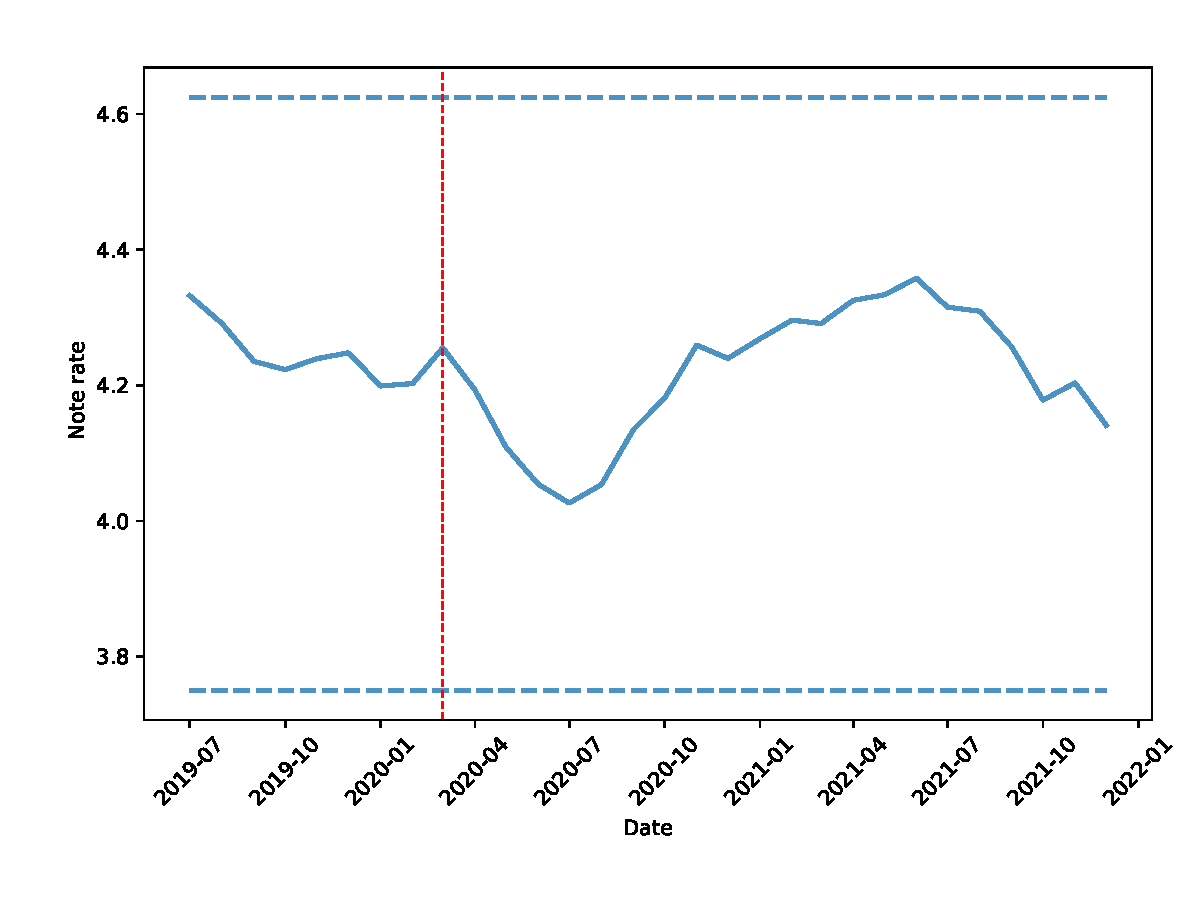
\includegraphics[width=0.998\textwidth]{../results/figures/NoteRate_mean_mat30_loan1_timeseries_nrmonthly_2.5_4_c35.0.pdf}
          \caption{ Coupon 3.5}
          \end{subfigure}
        \begin{subfigure}[b]{0.49\textwidth}
          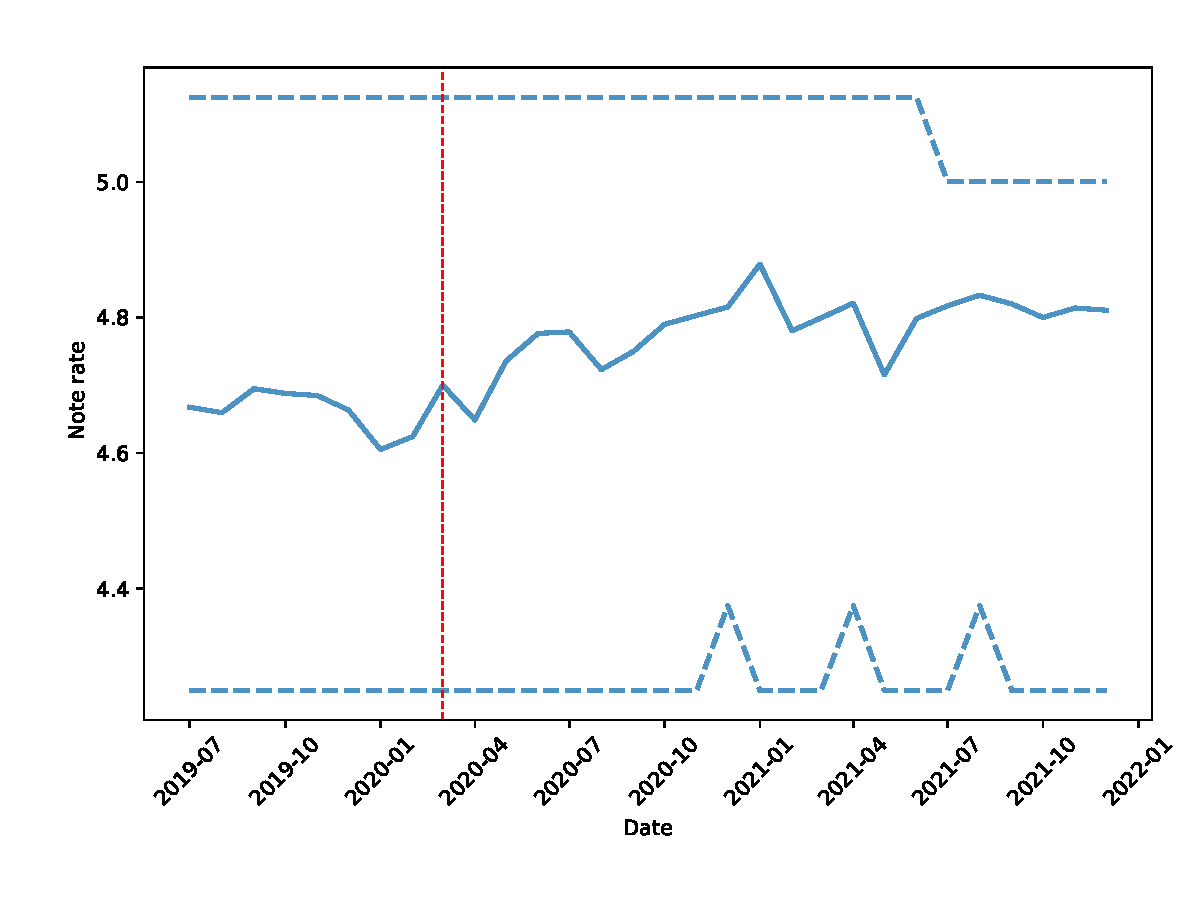
\includegraphics[width=0.998\textwidth]{../results/figures/NoteRate_mean_mat30_loan1_timeseries_nrmonthly_2.5_4_c40.0.pdf}
          \caption{ Coupon 4.0}
          \end{subfigure}
   \caption{Note rates by coupons over time} 
   \begin{minipage}{\textwidth}
      \footnotesize{\textit{Notes:} The figure shows the time series of auction outcomes for Conforming loans with a 30-year maturity.  The vertical line is March 1.}
      \end{minipage}
\end{figure}



\pagebreak
\subsection{Prices and Quantities}

The following figures show OB auctions mean, median higher bid, quantities, and the number of auctions that occurred daily from July 2019 to December 31st,  2021. We focus on 2.5, 3.0, 3.5 and 4.0 coupons. 

%April 30th, 2020.

\begin{figure}[h]
  \centering
  \begin{subfigure}[b]{0.49\textwidth}
      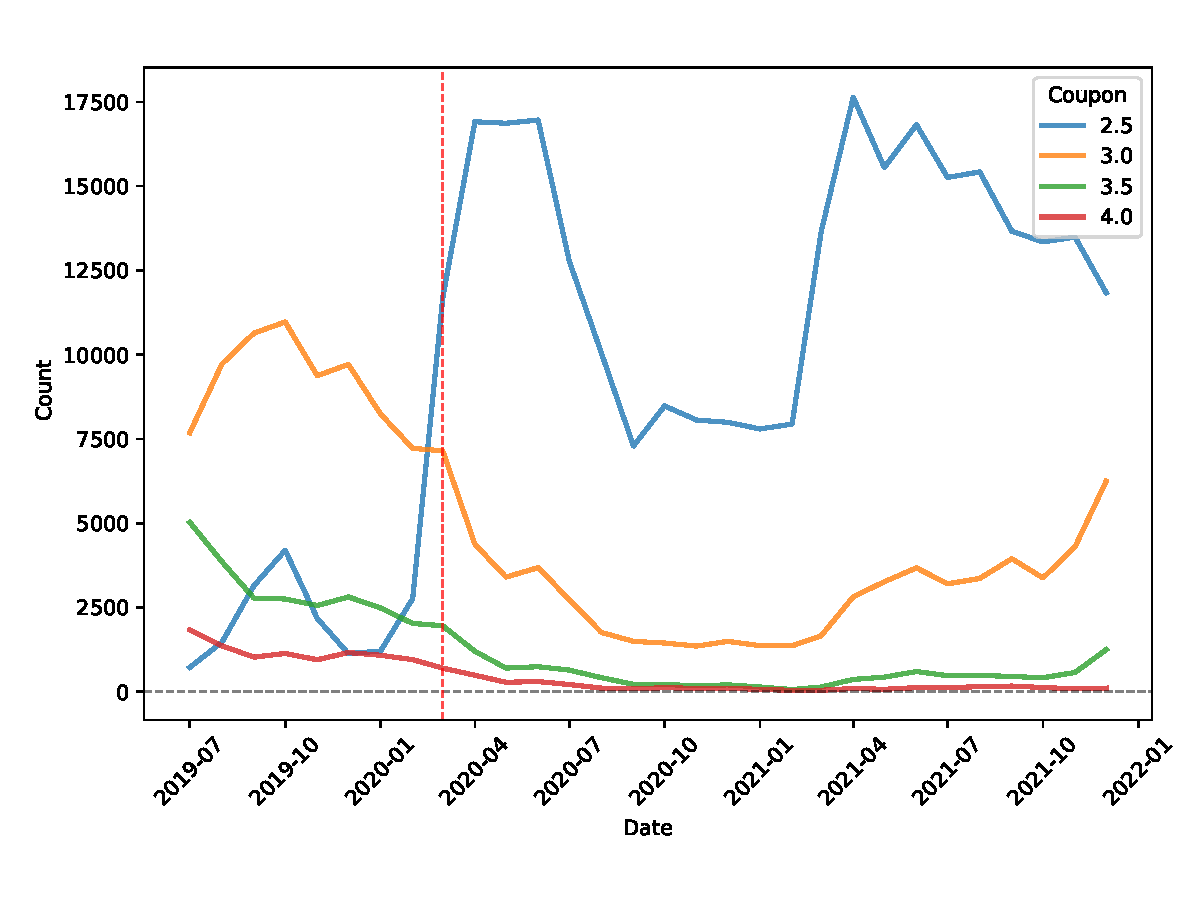
\includegraphics[width=0.998\textwidth]{../results/figures/winner_bid_count_mat30_loan1_timeseries_cpmonthly_2.5_4_.pdf}
      \caption{ Number of auctions}
     \end{subfigure}
     \begin{subfigure}[b]{0.49\textwidth}
      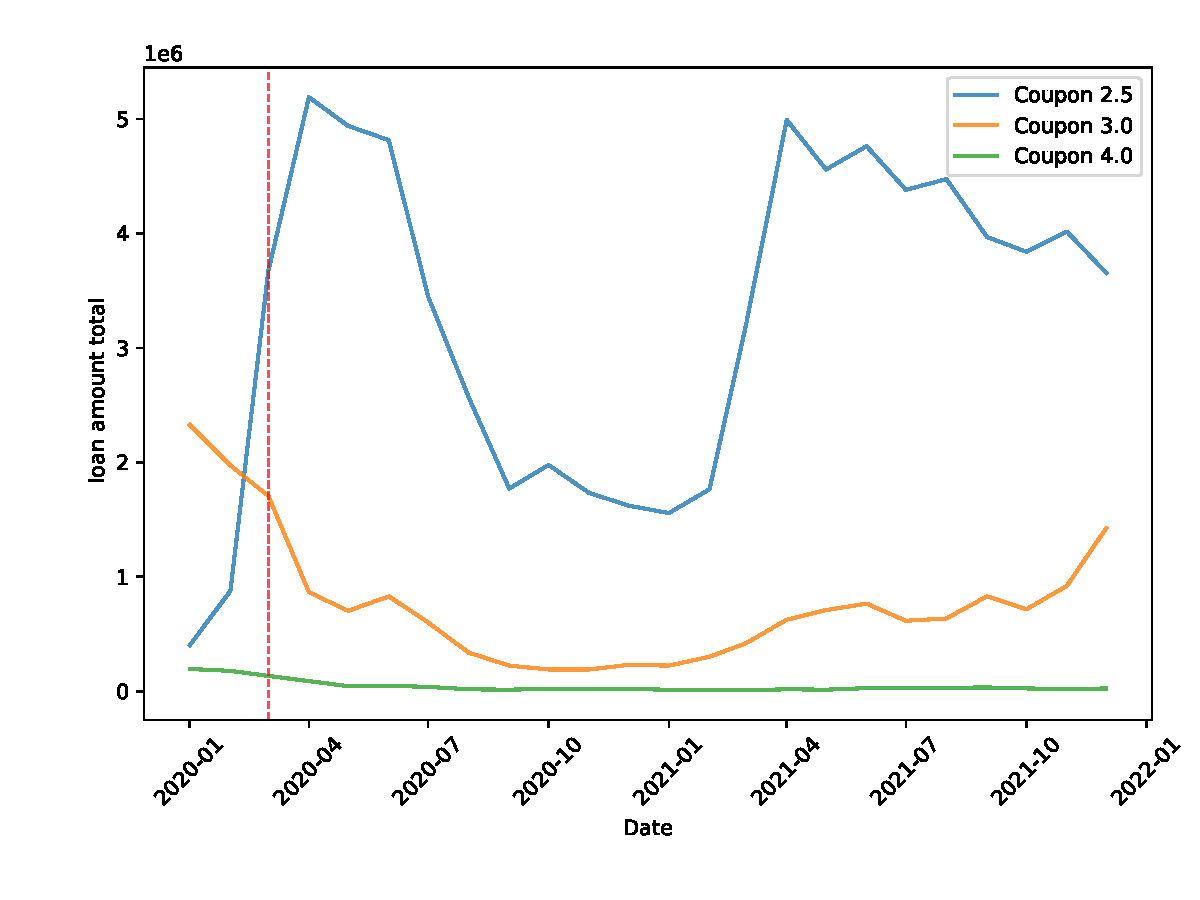
\includegraphics[width=0.998\textwidth]{../results/figures/LoanAmount_sum_mat30_loan1_timeseries_cpmonthly_2.5_4_.pdf}
      \caption{Loan amount}
     \end{subfigure}
     \begin{subfigure}[b]{0.49\textwidth}
      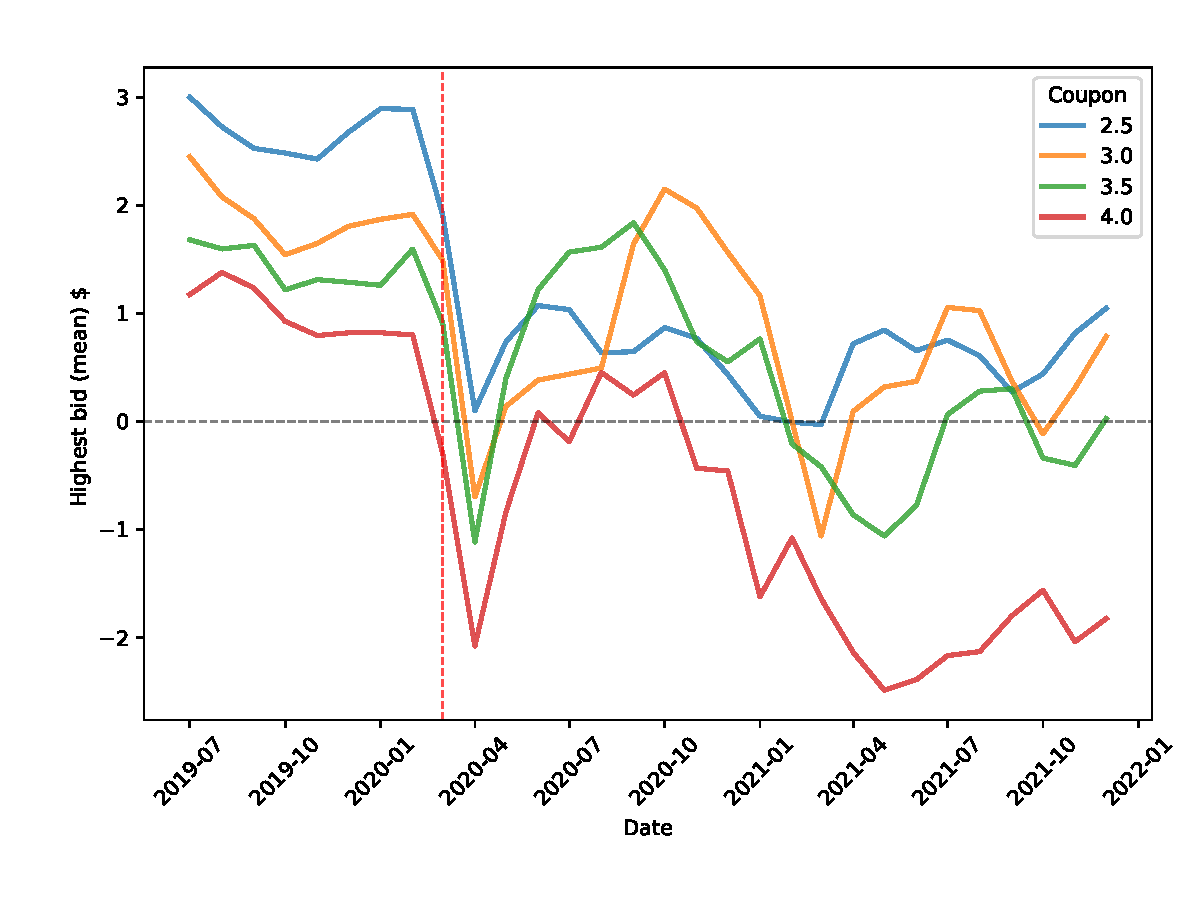
\includegraphics[width=0.998\textwidth]{../results/figures/winner_bid_mean_mat30_loan1_timeseries_cpmonthly_2.5_4__netbid.pdf}
      \caption{ Mean of highest net bid}
     \end{subfigure}
     \begin{subfigure}[b]{0.49\textwidth}
      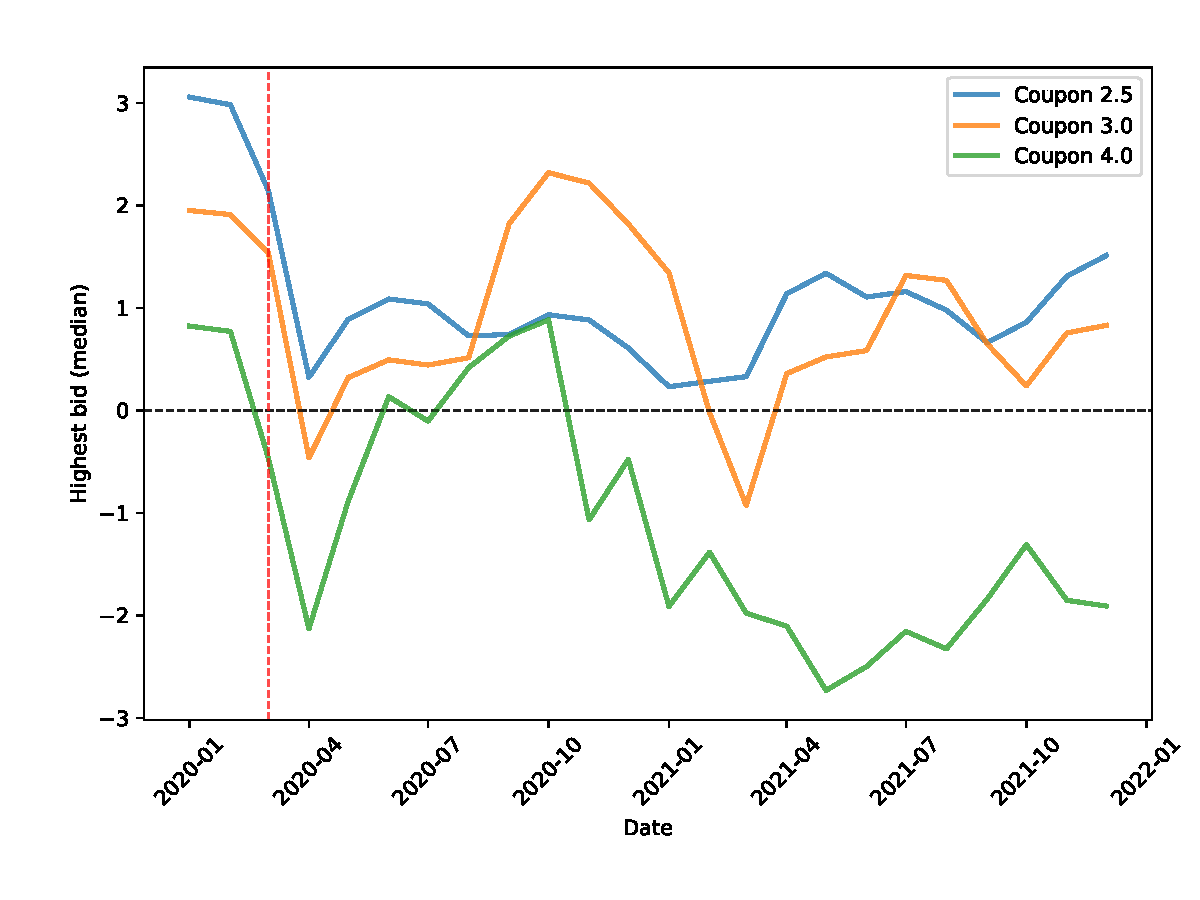
\includegraphics[width=0.998\textwidth]{../results/figures/winner_bid_median_mat30_loan1_timeseries_cpmonthly_2.5_4__netbid.pdf}
      \caption{ Median of highest net bid}
     \end{subfigure}
   \caption{OB auction outcomes. } 
   \begin{minipage}{\textwidth}
      \footnotesize{\textit{Notes:} The figure shows the time series of auction outcomes for Conforming loans with a 30-year maturity.  The vertical line is March 1. The net bid is calculated by subtracting the TBA Bloomberg price for the same coupon and two forward months from the OB auction price. }
      \end{minipage}
\end{figure}

\pagebreak
% \subsubsection{Comparison of note rates}

% \begin{figure}[h]
%   \centering
%   \begin{subfigure}[b]{0.49\textwidth}
%       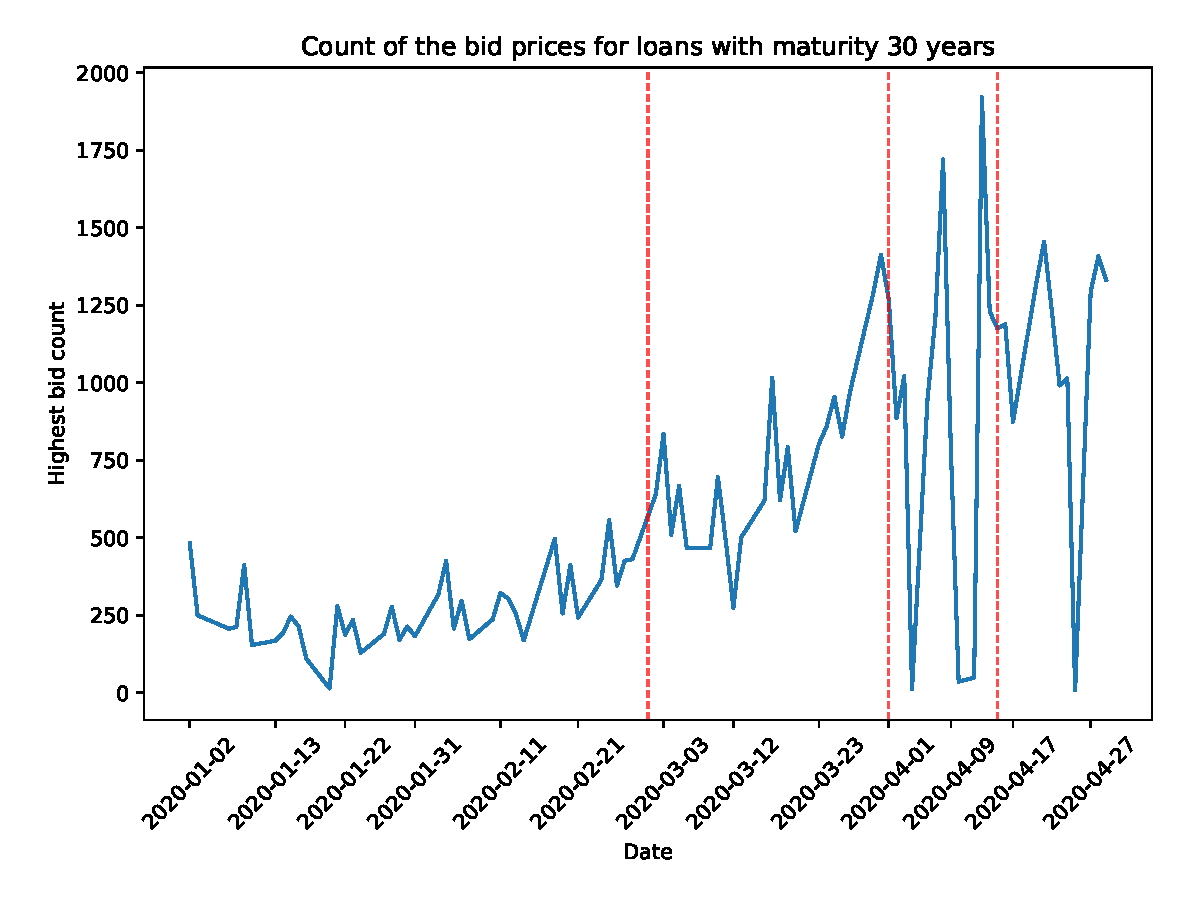
\includegraphics[width=0.998\textwidth]{../results/figures/winner_bid_count_mat30_loan1_timeseries_nr_3_3.75.pdf}
%       \caption{ Number of auctions}
%      \end{subfigure}
%      \begin{subfigure}[b]{0.49\textwidth}
%       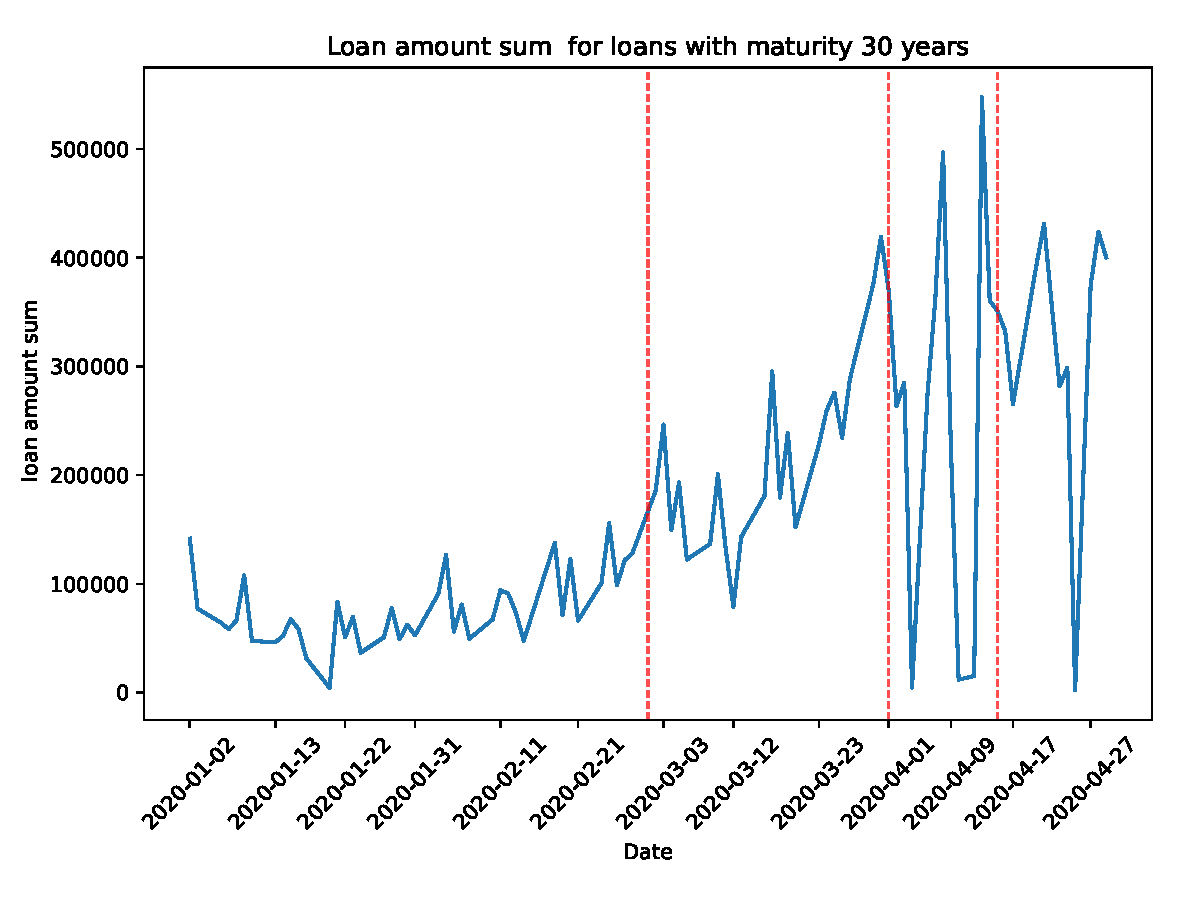
\includegraphics[width=0.998\textwidth]{../results/figures/LoanAmount_sum_mat30_loan1_timeseries_nr_3_3.75.pdf}
%       \caption{ Daily loan amount}
%      \end{subfigure}
%      \begin{subfigure}[b]{0.49\textwidth}
%       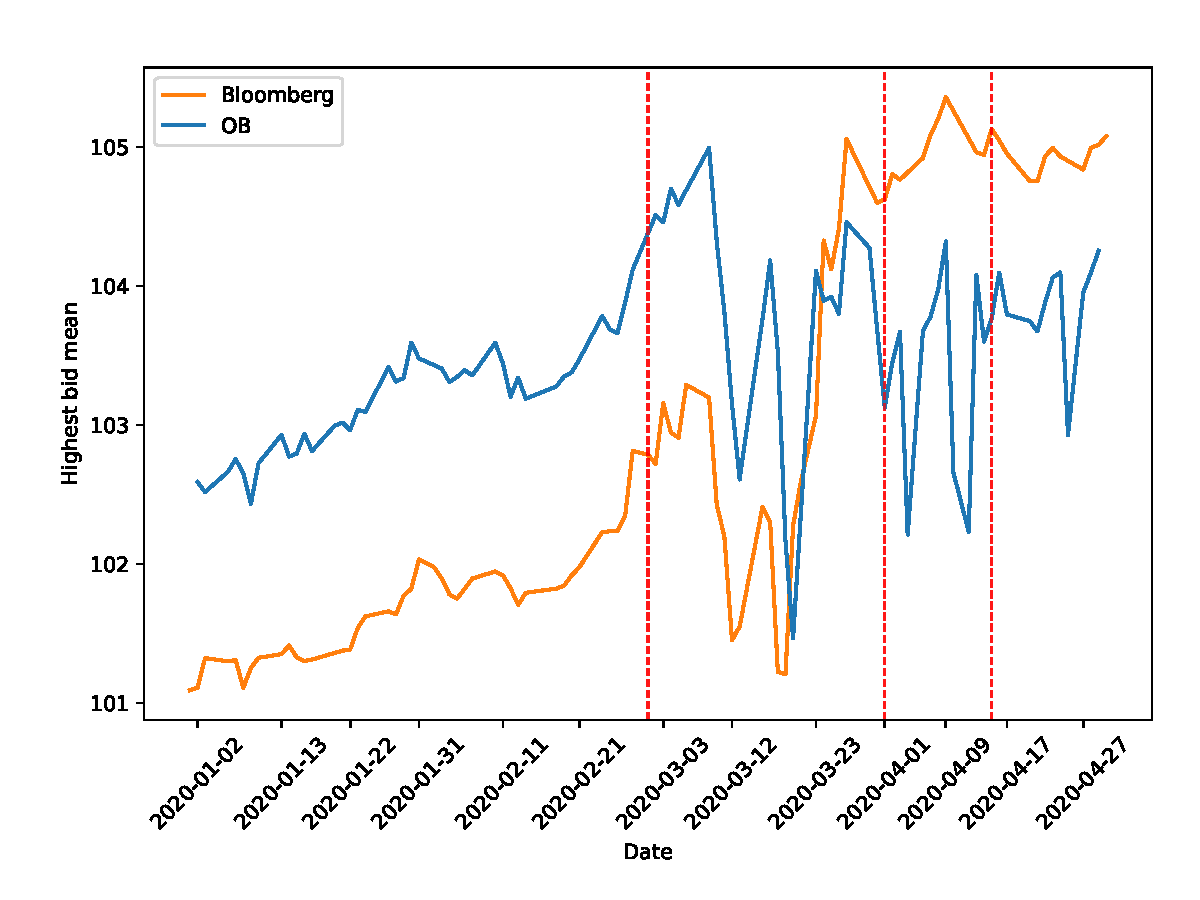
\includegraphics[width=0.998\textwidth]{../results/figures/w_winner_bid_mean_mat30_loan1_timeseries_nr_3_3.75.pdf}
%       \caption{ Weighted mean of highest bid}
%      \end{subfigure}
%      \begin{subfigure}[b]{0.49\textwidth}
%       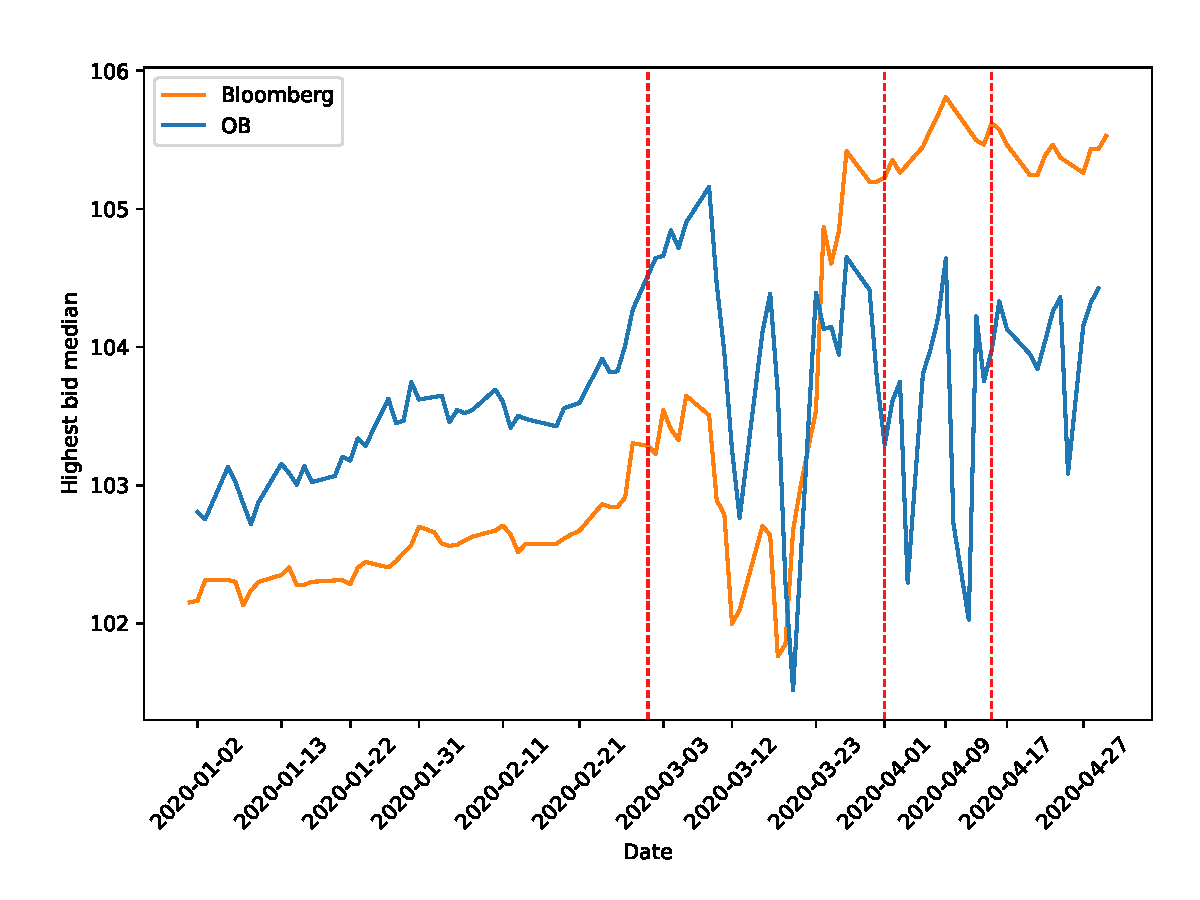
\includegraphics[width=0.998\textwidth]{../results/figures/winner_bid_median_mat30_loan1_timeseries_nr_3_3.75.pdf}
%       \caption{ Median of highest bid}
%      \end{subfigure}
%    \caption{OB auction outcomes for note rates between 3\% and 3.75\%}
%    \begin{minipage}{\textwidth}
%       \footnotesize{\textit{Notes:} The figure shows time series of auction outcomes for Conforming loans with a 30-year maturity. The vertical line is March 1. For reference, Bloomberg TBA prices are aggregated for all forward months and coupons between 2.5, 3, and 3.5. } 
%       \end{minipage}
% \end{figure}

% \pagebreak

% \begin{figure}[h]
%   \centering
%   \begin{subfigure}[b]{0.49\textwidth}
%       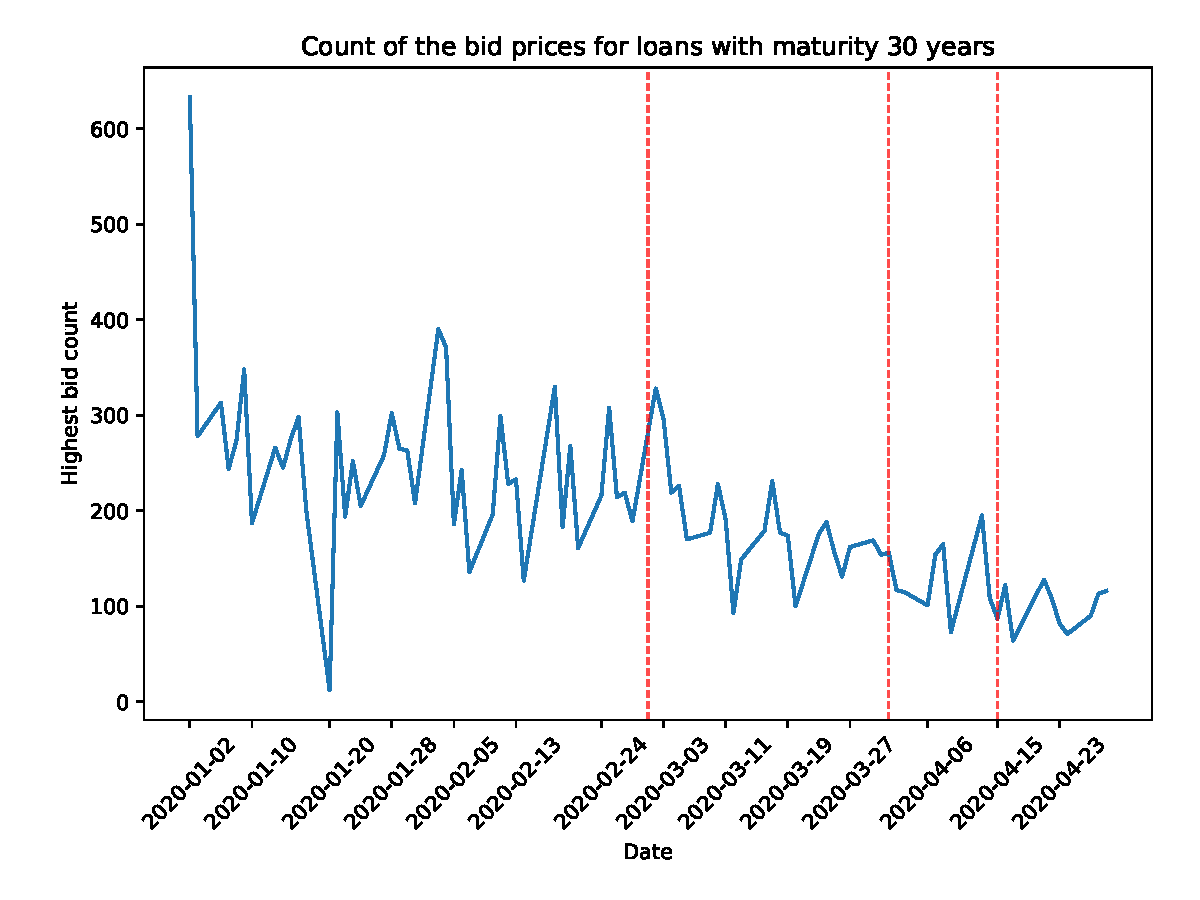
\includegraphics[width=0.998\textwidth]{../results/figures/winner_bid_count_mat30_loan1_timeseries_nr_4_4.75.pdf}
%       \caption{ Number of auctions}
%      \end{subfigure}
%      \begin{subfigure}[b]{0.49\textwidth}
%       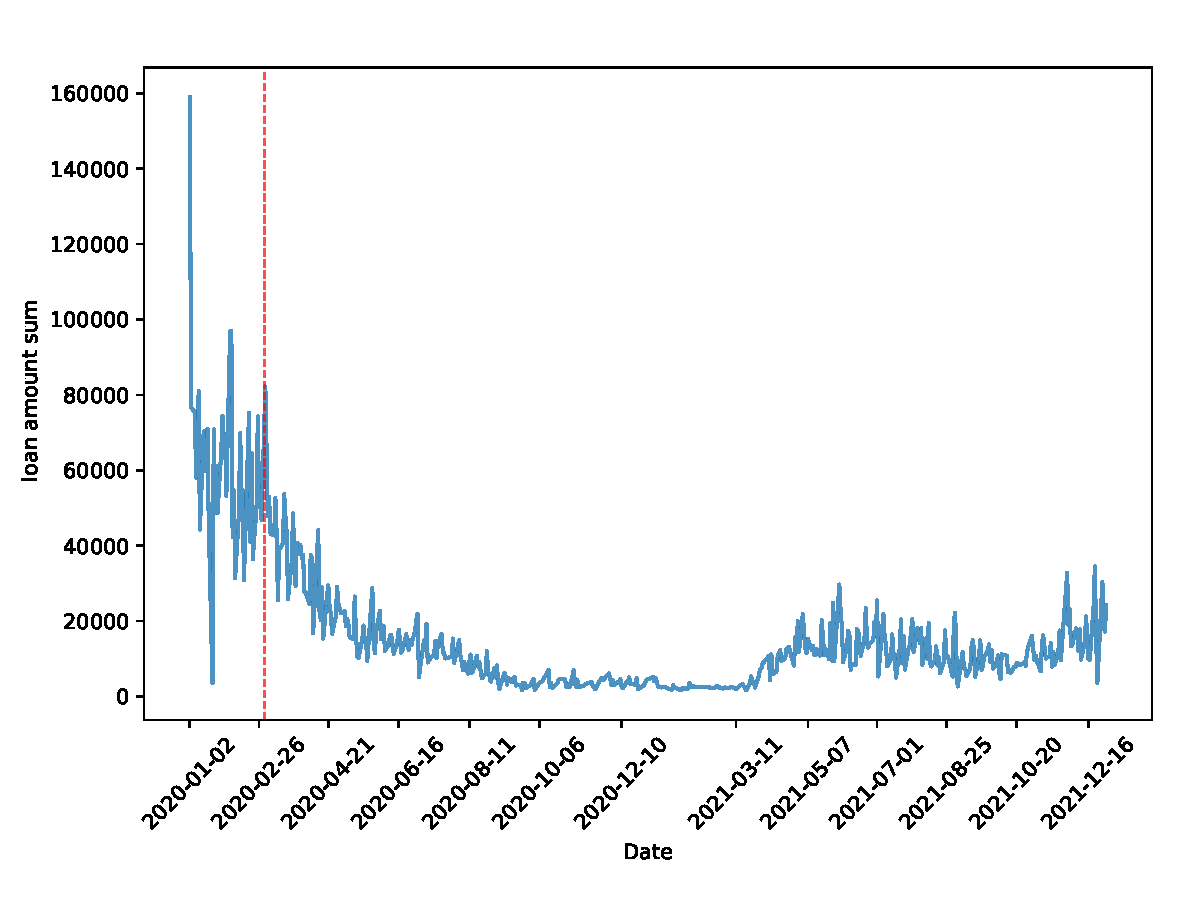
\includegraphics[width=0.998\textwidth]{../results/figures/LoanAmount_sum_mat30_loan1_timeseries_nr_4_4.75.pdf}
%       \caption{ Daily loan amount}
%      \end{subfigure}
%      \begin{subfigure}[b]{0.49\textwidth}
%       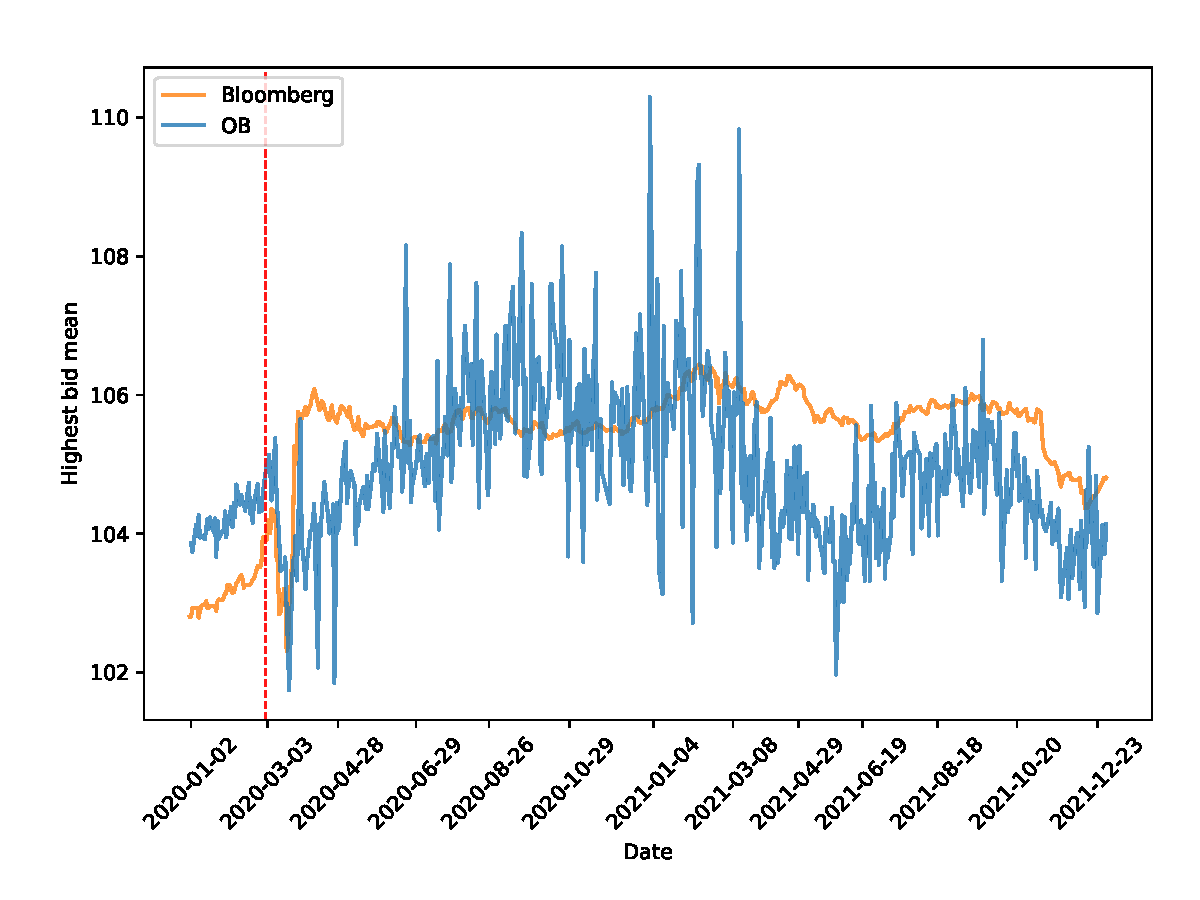
\includegraphics[width=0.998\textwidth]{../results/figures/w_winner_bid_mean_mat30_loan1_timeseries_nr_4_4.75.pdf}
%       \caption{ Weighted mean of highest bid}
%      \end{subfigure}
%      \begin{subfigure}[b]{0.49\textwidth}
%       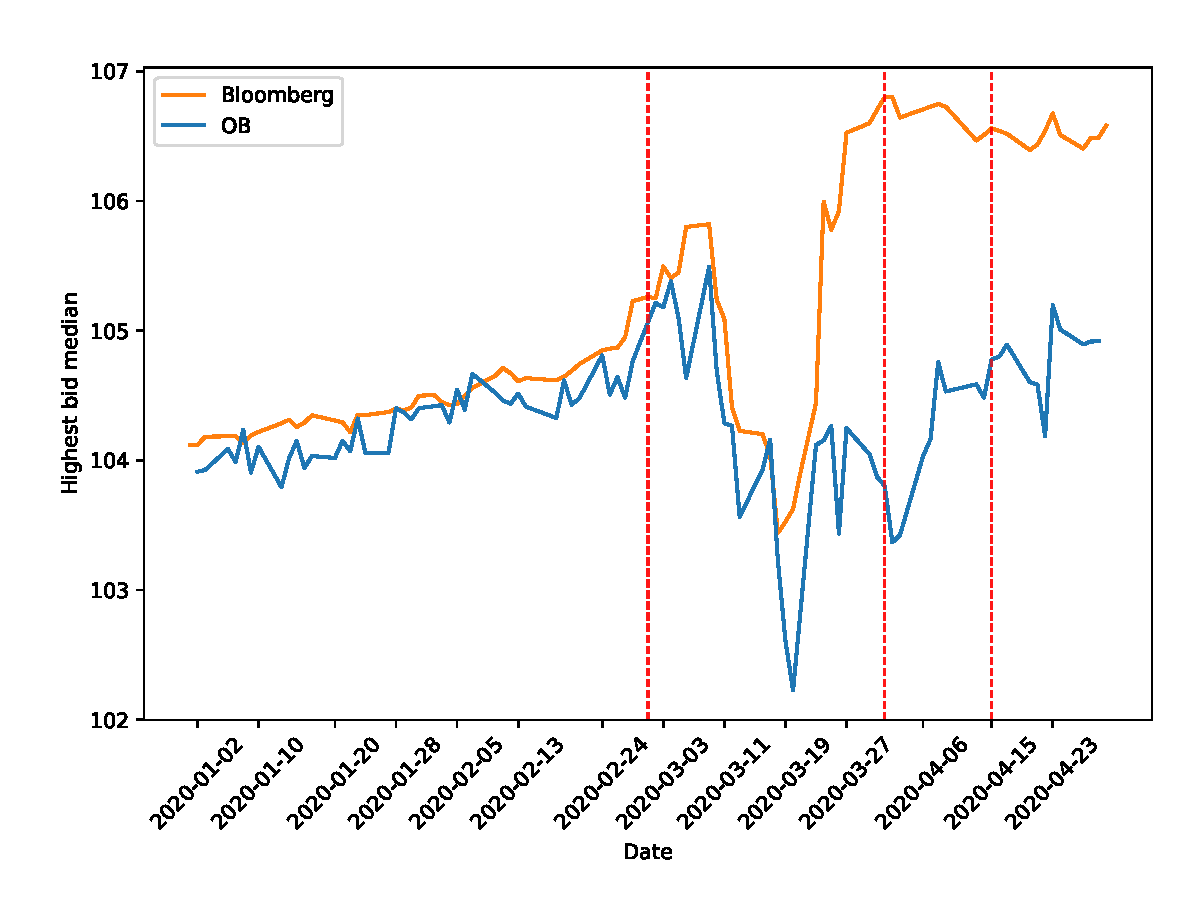
\includegraphics[width=0.998\textwidth]{../results/figures/winner_bid_median_mat30_loan1_timeseries_nr_4_4.75.pdf}
%       \caption{ Median of highest bid}
%      \end{subfigure}
%    \caption{OB auction outcomes for note rates between 4\% and 4.75\%}
%    \begin{minipage}{\textwidth}
%       \footnotesize{\textit{Notes:} The figure shows the time series of auction outcomes for Conforming loans with a 30-year maturity.  The vertical line is March 1. For reference, Bloomberg TBA prices are aggregated for all forward months and coupons 3.5, 4, and 4.5. } 
%       \end{minipage}
% \end{figure}

\pagebreak

\subsection{Distress signs in the OB auctions}

Below, we show distress and illiquidity measures in the OB auctions during the early Covid period. The variables are defined as follows:
\begin{itemize}
\item \textbf{Days to auction}: Number of days between the auction date and the date the loan originated.
\item \textbf{Number of participants}: Number of participants in the auction.
\item  \textbf{Winner Sell rate:} Rate to which the loan is sold to the auction participant with the highest bid. Since the highest bid is not always the winning bid because sometimes the winner's bid is missing, and other times the committed investor is not the one with the highest bid. 
\item \textbf{Number of bulk bidders:} Bulk bids are bids where delivery method bulk.
\end{itemize}
\begin{figure}[h]
  \centering
  \begin{subfigure}[b]{0.49\textwidth}
      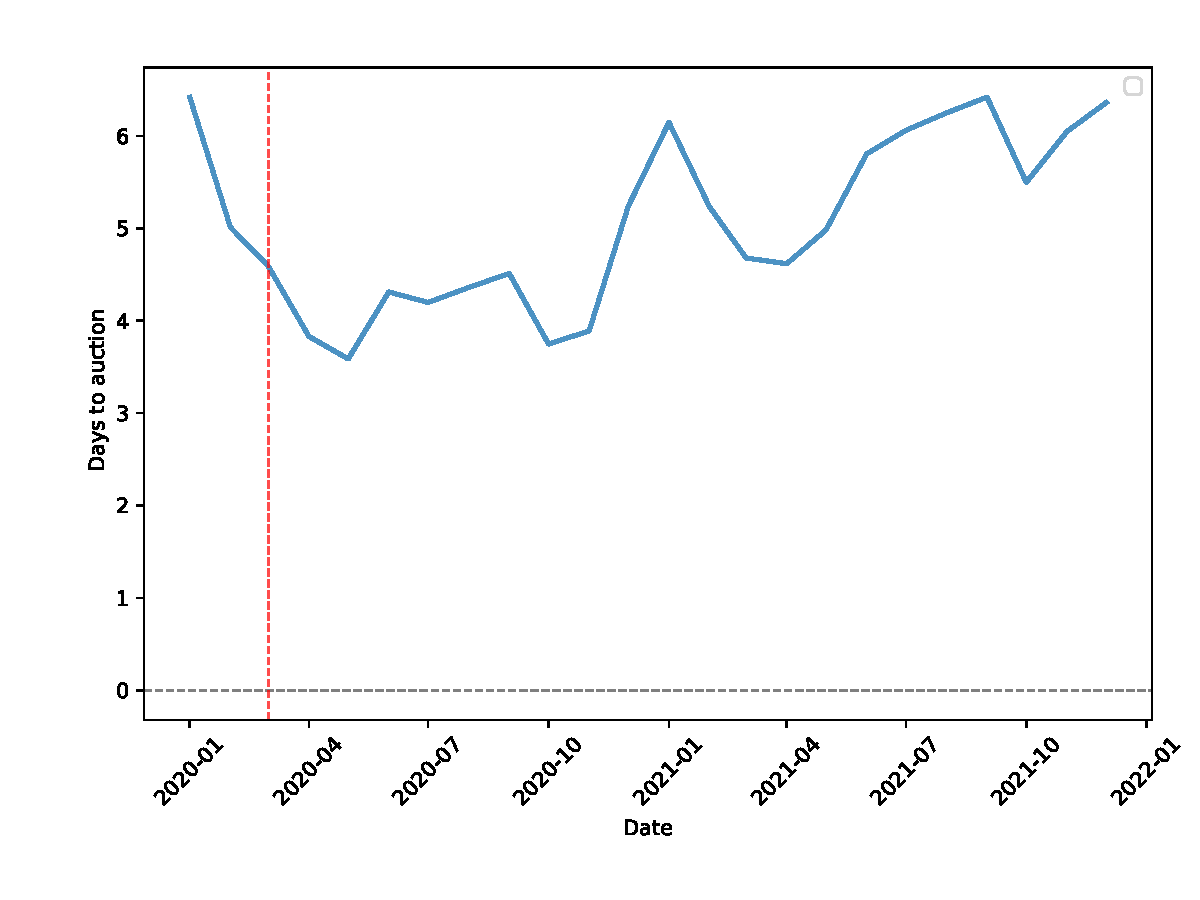
\includegraphics[width=0.998\textwidth]{../results/figures/DaysToAuction_mean_mat30_loan1_timeseries_nrmonthly_2.5_4_.pdf}
      \caption{Days to auction}
     \end{subfigure}
     \begin{subfigure}[b]{0.49\textwidth}
      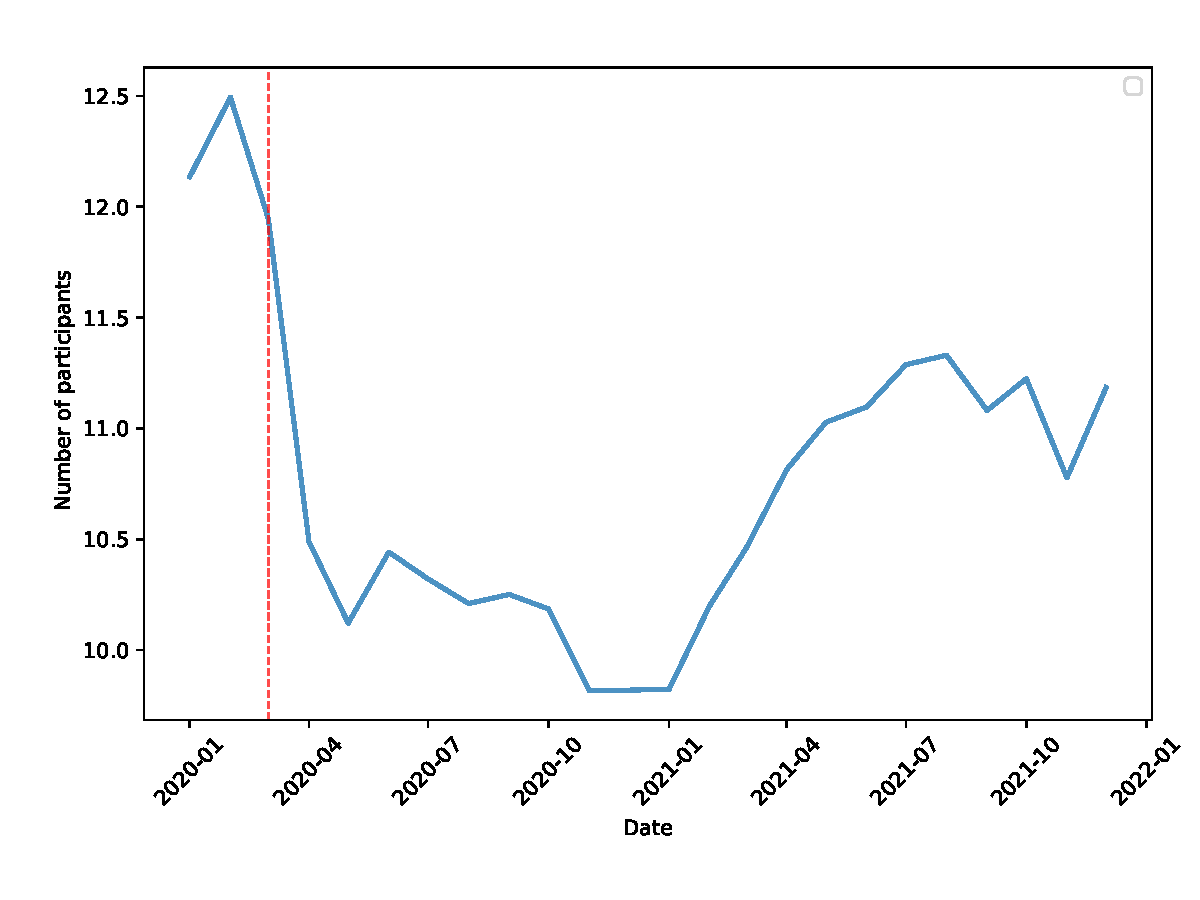
\includegraphics[width=0.998\textwidth]{../results/figures/Number of Participants_mean_mat30_loan1_timeseries_nrmonthly_2.5_4_.pdf}
      \caption{ Number of participants}
     \end{subfigure}
     \begin{subfigure}[b]{0.49\textwidth}
      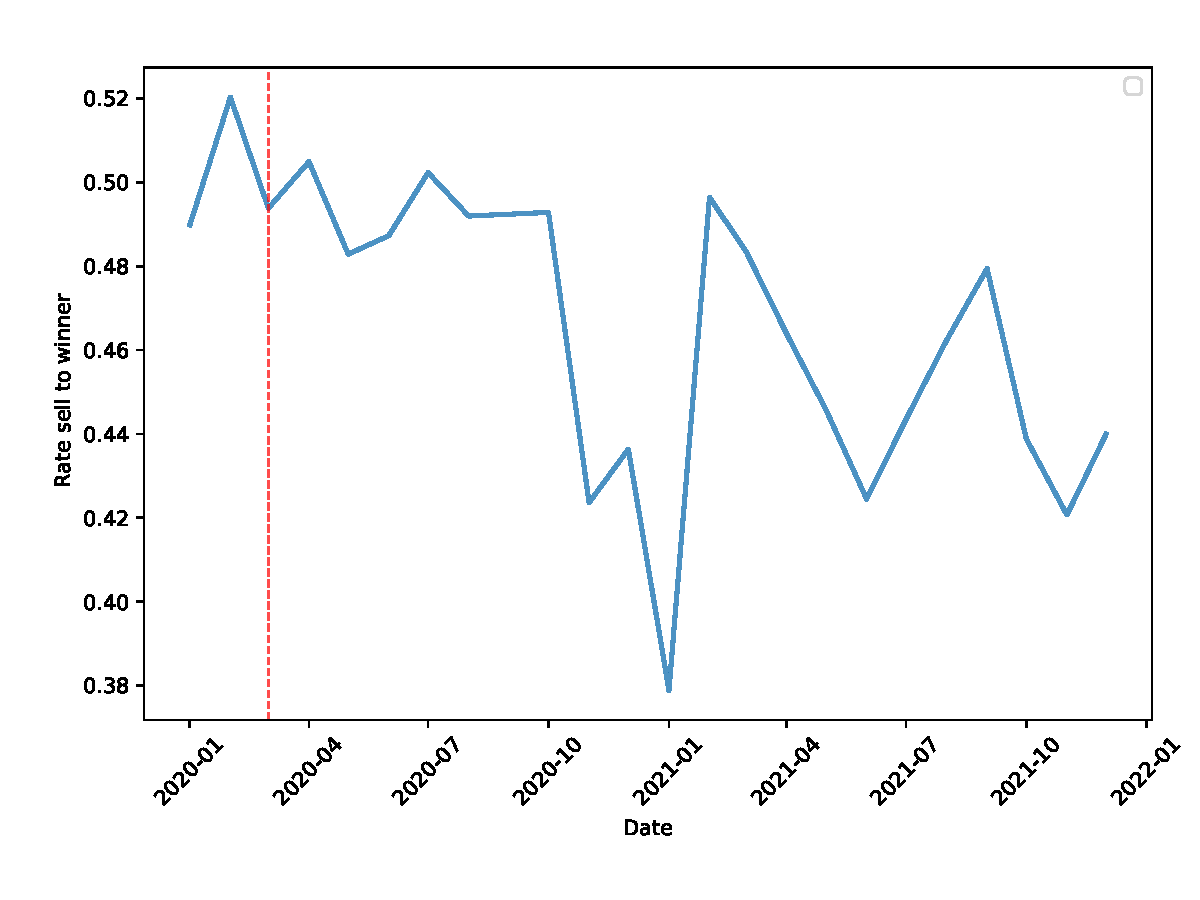
\includegraphics[width=0.998\textwidth]{../results/figures/dummy_sell_winner_mean_mat30_loan1_timeseries_nrmonthly_2.5_4_.pdf}
      \caption{ Winner sell rate}
      \end{subfigure}
      \begin{subfigure}[b]{0.49\textwidth}
        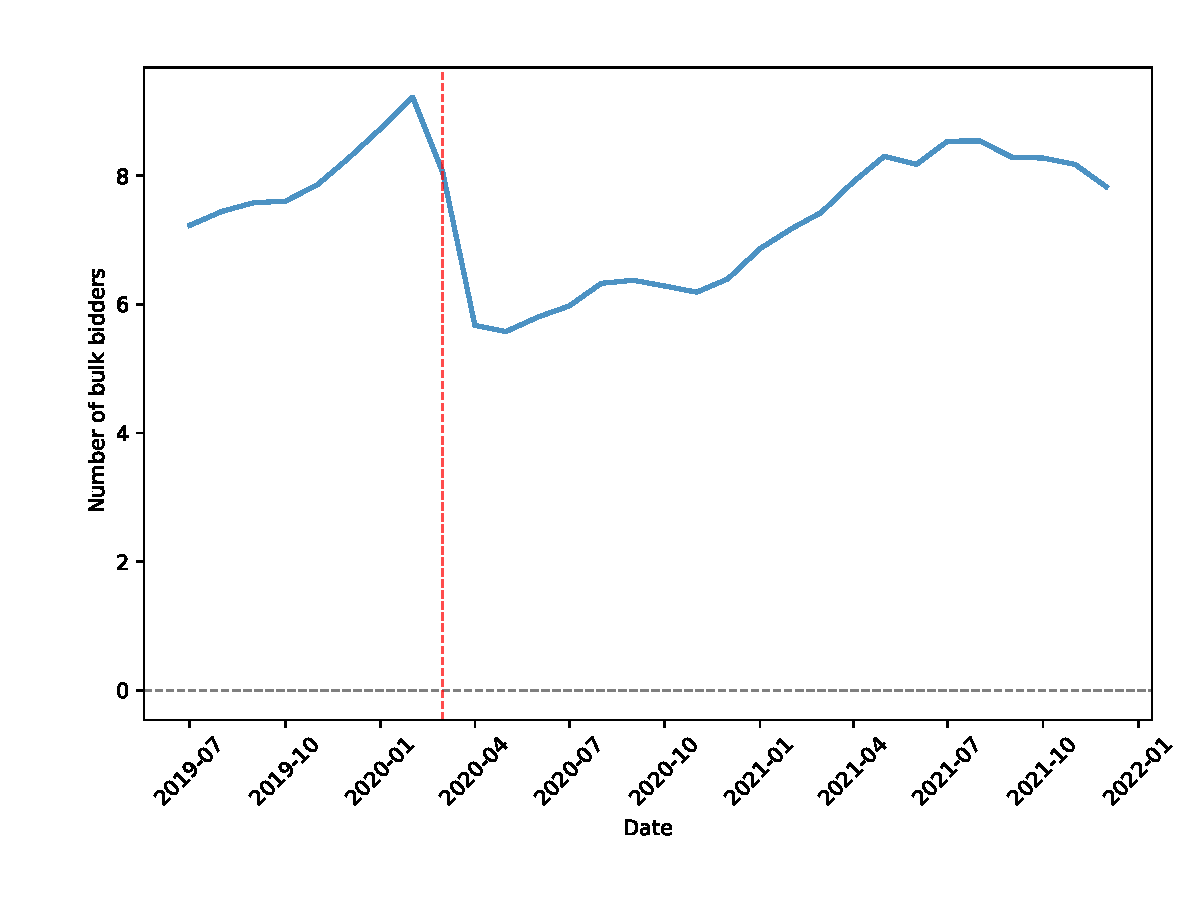
\includegraphics[width=0.998\textwidth]{../results/figures/Number of Bulk Bidders_mean_mat30_loan1_timeseries_nrmonthly_2.5_4_.pdf}
        \caption{ Number of bulk bidders}
       \end{subfigure}
     \caption{OB auction outcomes } 
   \begin{minipage}{\textwidth}
      \footnotesize{\textit{Notes:} The figure shows time series of auction outcomes for Conforming loans with a 30-year maturity. The vertical line is March 1.  } 
      \end{minipage}
\end{figure}

\pagebreak
\subsubsection{Bulk bidders}

Now, we examine the number of bulk bidders in the OB auctions and the number of participants that are banks.

\begin{figure}[h]
  \centering
  \begin{subfigure}[b]{0.49\textwidth}
    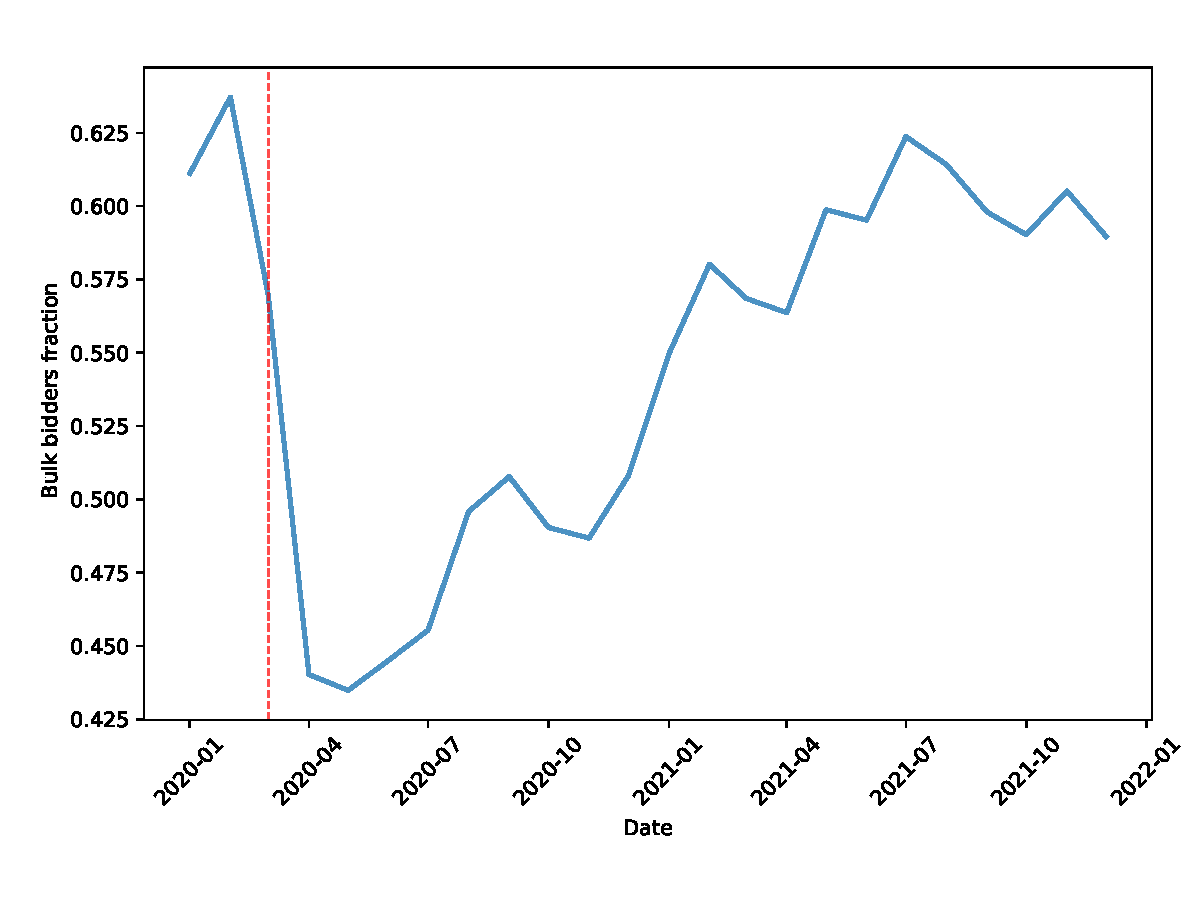
\includegraphics[width=0.998\textwidth]{../results/figures/bulk_bidders_fraction_mean_mat30_loan1_timeseries_nrmonthly_2.5_4_.pdf}
    \caption{ Fraction of bulk bidders}
   \end{subfigure}
     \begin{subfigure}[b]{0.49\textwidth}
      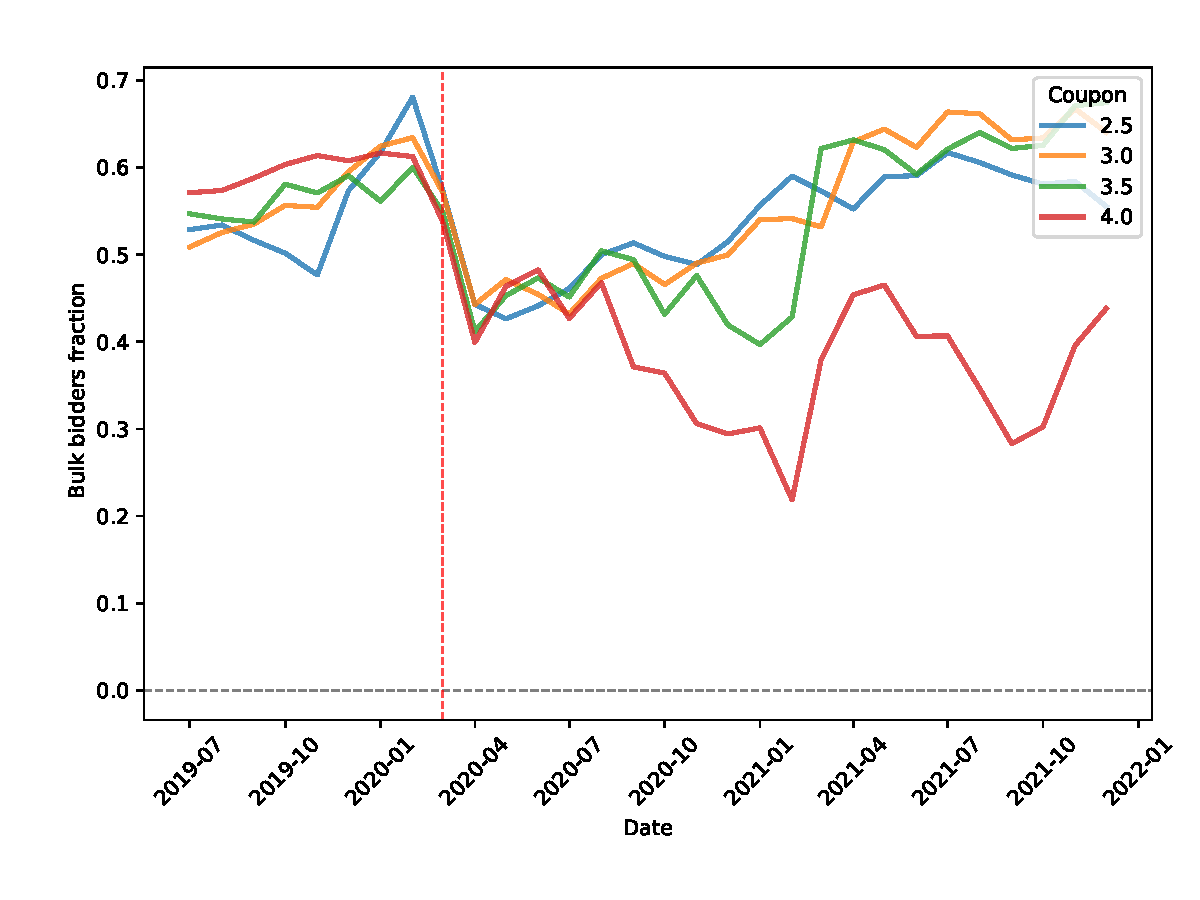
\includegraphics[width=0.998\textwidth]{../results/figures/bulk_bidders_fraction_mean_mat30_loan1_timeseries_cpmonthly_2.5_4_.pdf}
      \caption{ Fraction of bulk bidders by coupon}
     \end{subfigure}
     \begin{subfigure}[b]{0.49\textwidth}
      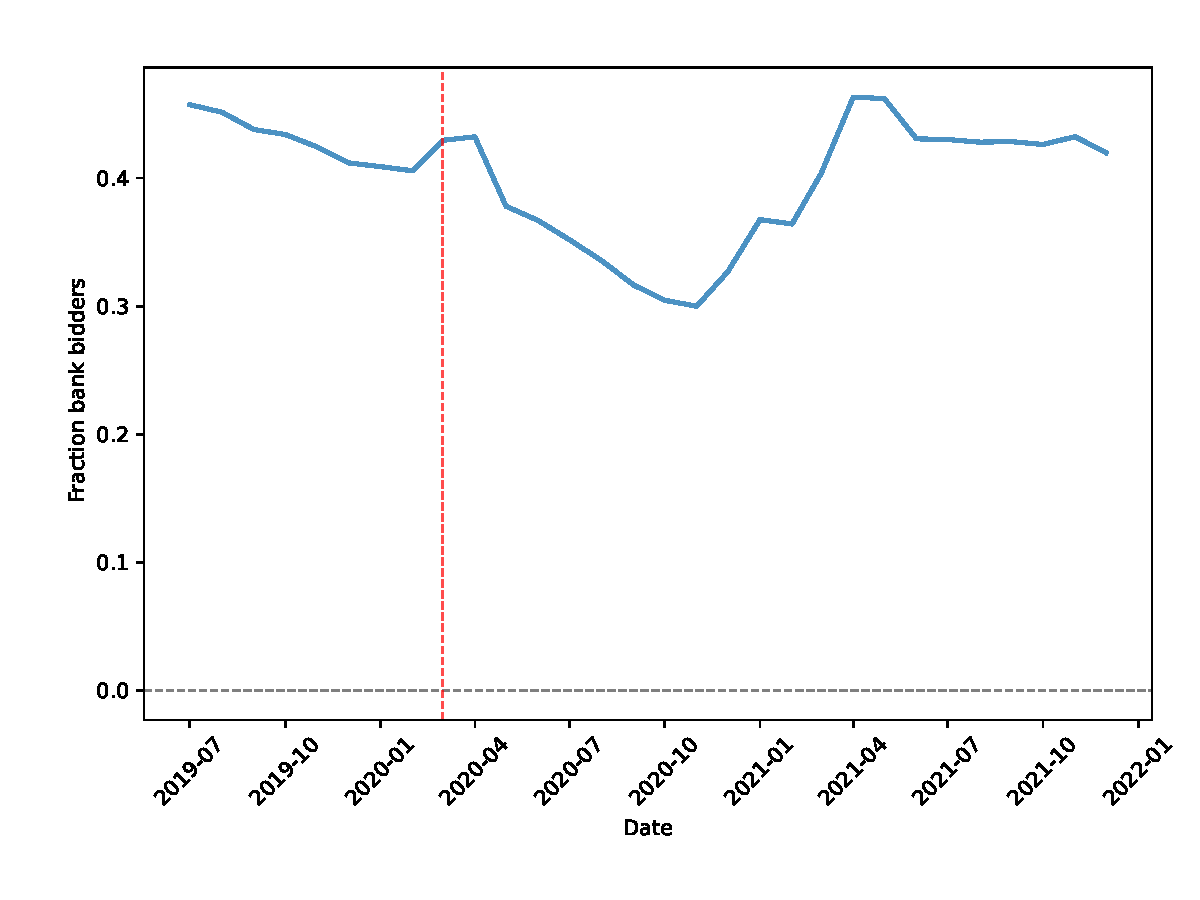
\includegraphics[width=0.998\textwidth]{../results/figures/fraction_banks_mean_mat30_loan1_timeseries_nrmonthly_2.5_4_.pdf}
      \caption{  Number of bank bidders}
     \end{subfigure}
       \begin{subfigure}[b]{0.49\textwidth}
        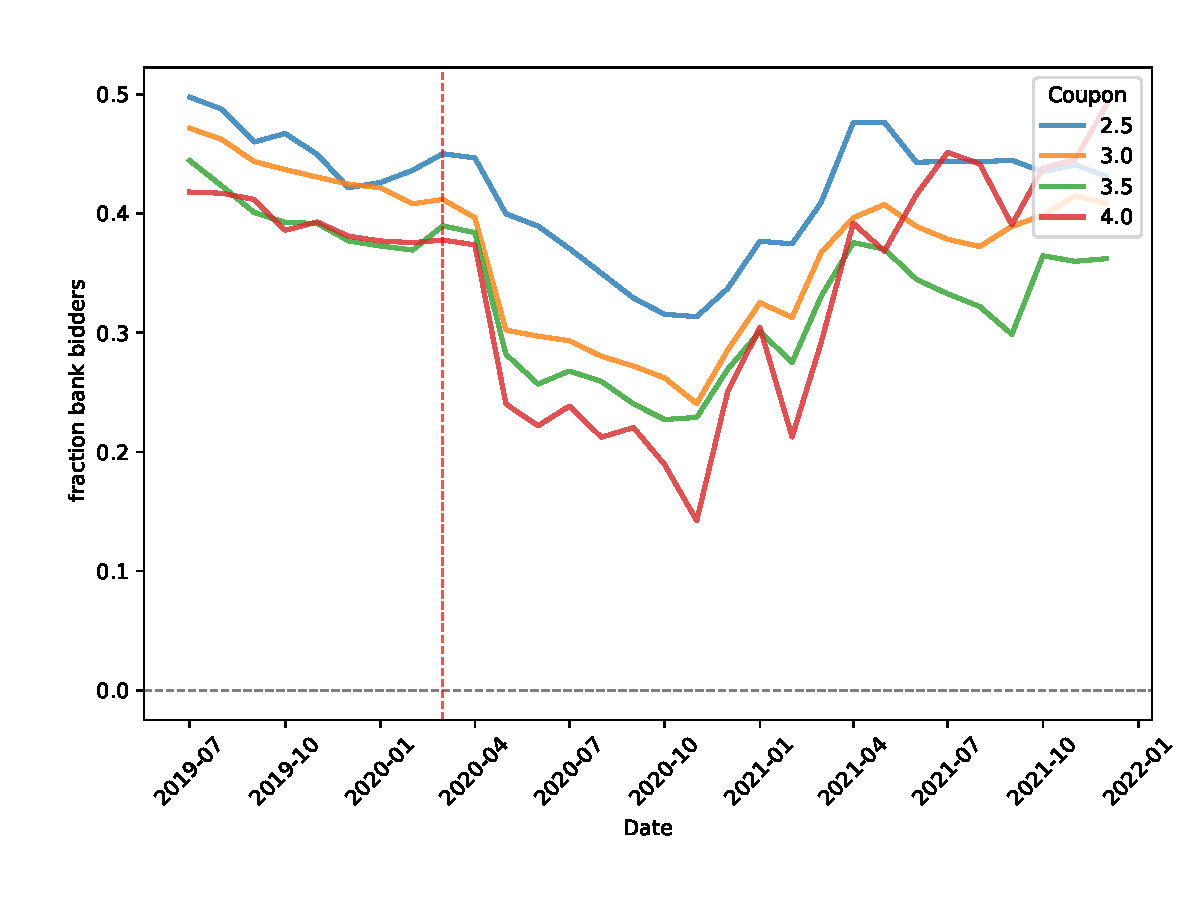
\includegraphics[width=0.998\textwidth]{../results/figures/fraction_banks_mean_mat30_loan1_timeseries_cpmonthly_2.5_4_.pdf}
        \caption{ Fraction of the nuber of bank bidders by coupon}
       \end{subfigure}
     \caption{Bulk bidders and bank participants} 
   \begin{minipage}{\textwidth}
      \footnotesize{\textit{Notes:} The figure shows time series of auction outcomes for Conforming loans with a 30-year maturity. The vertical line is March 1.  } 
      \end{minipage}
\end{figure}


\pagebreak
\subsection{GSE response }

 In this section, we show the GSE response to the covid crisis. The variables are defined as follows:
\begin{itemize}
% \item \textbf{Number of Enterprise Bids}: Number of bids per auction submitted by the GSEs (Fannie and Freddie).
\item \textbf{Fraction of loans sold to GSE}: Fraction of loans sold to the GSEs.
\item \textbf{GSE highest bid}: Highest bid in an auction where the GSE is the committed investor.
\end{itemize}

\begin{figure}[h]
  \centering
  \begin{subfigure}[b]{0.49\textwidth}
      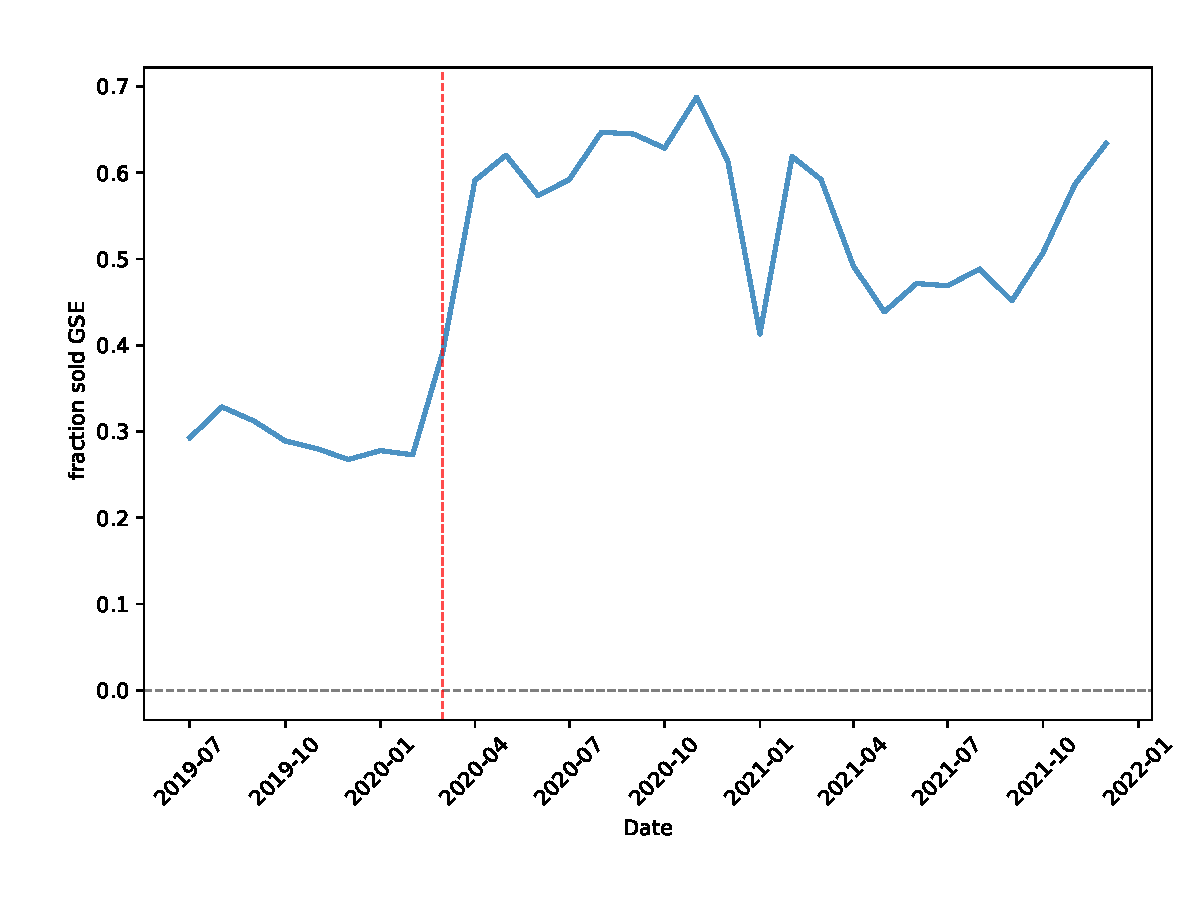
\includegraphics[width=0.998\textwidth]{../results/figures/sold_GSE_mean_mat30_loan1_timeseries_nrmonthly_2.5_4_.pdf}
      \caption{Fraction loans sold GSE in OB }
     \end{subfigure}
     \begin{subfigure}[b]{0.49\textwidth}
      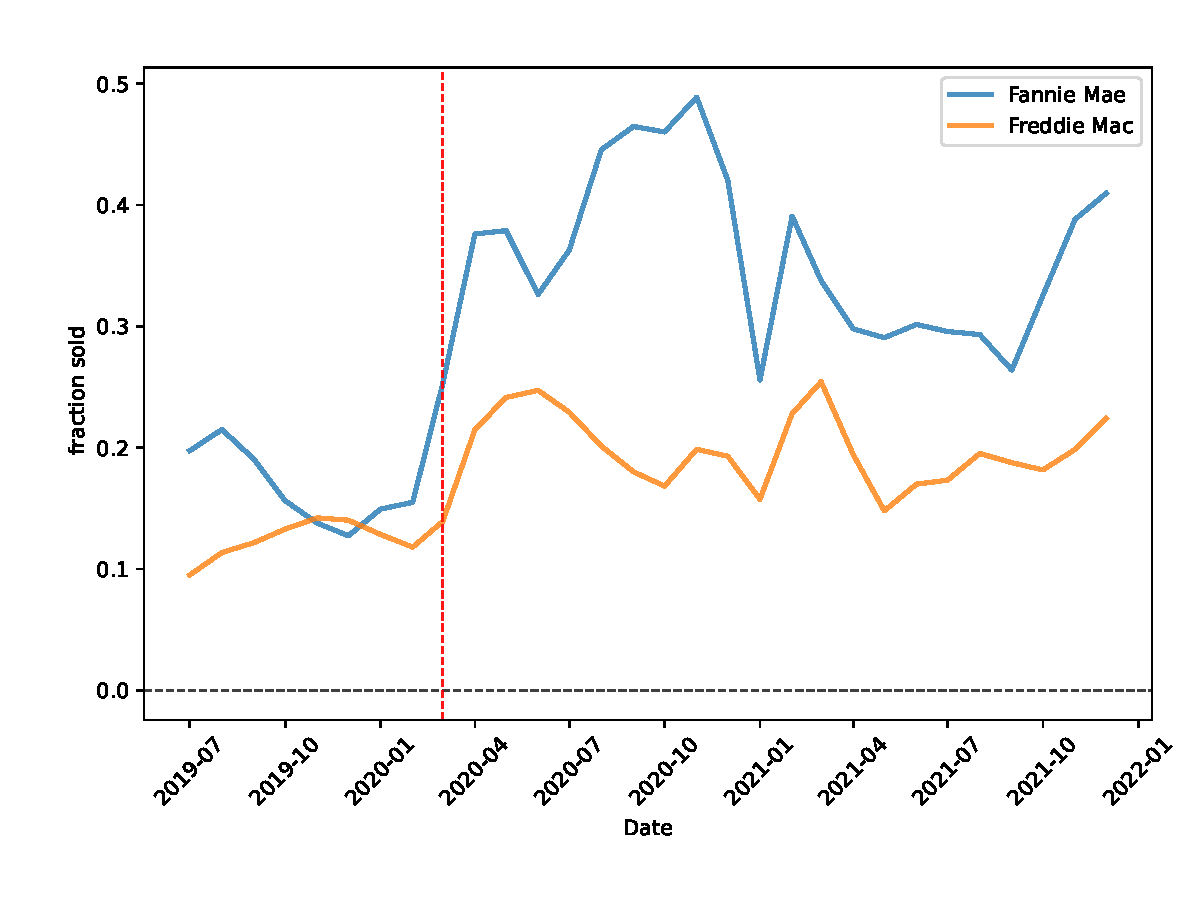
\includegraphics[width=0.998\textwidth]{../results/figures/sold_FreddieBid_mean_mat30_loan1_timeseries_nrmonthly_2.5_4_.pdf}
      \caption{ Fraction of loans sold to GSE by enterprise }\label{fig:gse_loans}
     \end{subfigure}
     \caption{OB auction  GSE response } 
   \begin{minipage}{\textwidth}
      \footnotesize{\textit{Notes:} The figure shows time series of auction outcomes for Conforming loans with a 30-year maturity. The vertical line is March 1.  } 
      \end{minipage}
\end{figure}

\pagebreak
\subsubsection{GSE bids difference}

Next, to understand the differences between Fannie and Freddie in \ref{fig:gse_loans}, we plot the difference between the highest bids in auctions where Fannie is the committed investor and Freddie is the committed investor. 

\begin{figure}[h]
  \centering
  \begin{subfigure}[b]{0.49\textwidth}
      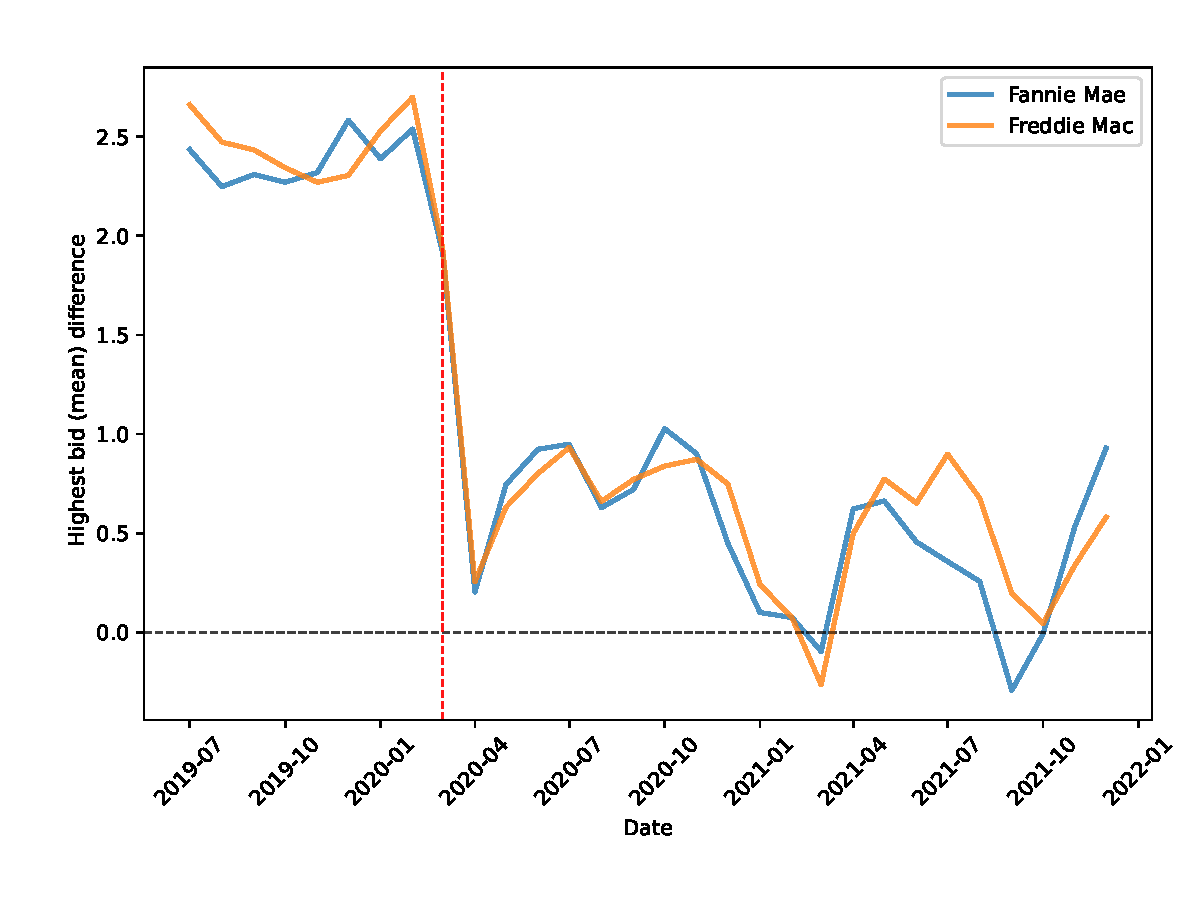
\includegraphics[width=0.998\textwidth]{../results/figures/price_freddie_mean_mat30_loan1_timeseries_nrmonthly_2.5_4_byGSE_c25.pdf}
      \caption{Average bids for Freddie and Fannie} % Todo: Have 2.5 loan
     \end{subfigure}
     \begin{subfigure}[b]{0.49\textwidth}
      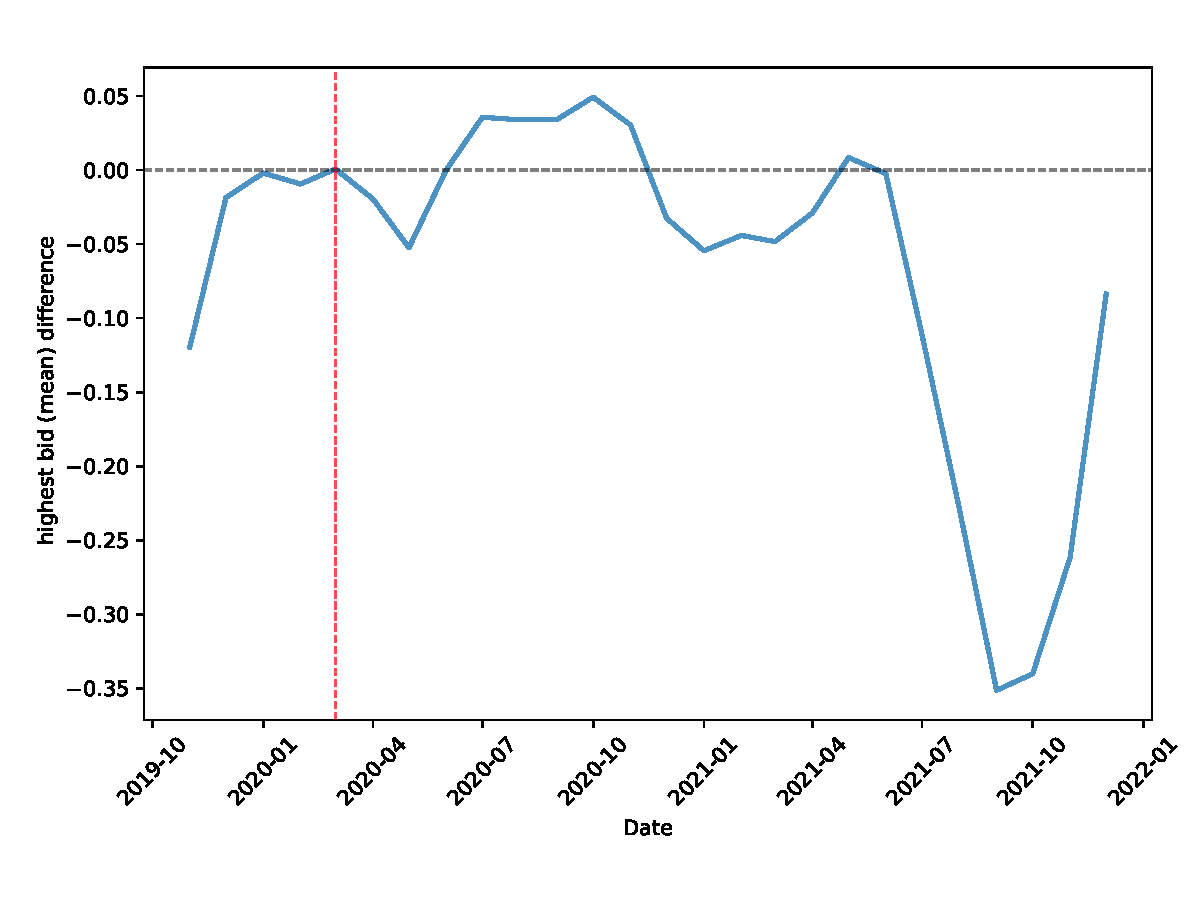
\includegraphics[width=0.998\textwidth]{../results/figures/price_diff_ma_mat30_loan1_timeseries_nrmonthly_2.5_4_diffFF_ma5_c25.pdf}
      \caption{ Bid difference between Freddie and Fannie.}
     \end{subfigure}
     \caption{OB auction  GSE response for coupon 2.5 } 
   \begin{minipage}{\textwidth}
      \footnotesize{\textit{Notes:} The figure shows time series of auction outcomes for Conforming loans with a 30-year maturity. The vertical line is March 1.  } 
      \end{minipage}
\end{figure}

\pagebreak
\subsubsection{Comparison GSE vs non-GSE}

Now we compare the highest bids of the auctions when the GSE is the committed investor and when the GSE is not the committed investor. More formally, we define: 

\begin{itemize}
  \item \textbf{auction transaction: } One of the non-GSE participants is the committed investor and the bid is in the sample. For 52 \% of the transactions, a non-GSE is the committed investor, and 7 \% of the time the bid is not in the sample. These observations are eliminated from the analysis.
  \item \textbf{cash window transaction: } The GSE is the committed investor. These are 48 \% of the transactions. All highest bids are included in the analysis. 
\end{itemize}

See ideally, we will plot the accepted bids, but these are not always in the data. Actually, 27 \% of auctions for this type of loan do not have the committer investors bid (70 \%  of times the bid is not in sample the GSE is the committed investor). 


\begin{figure}[h]
  \centering
     \begin{subfigure}[b]{0.49\textwidth} 
      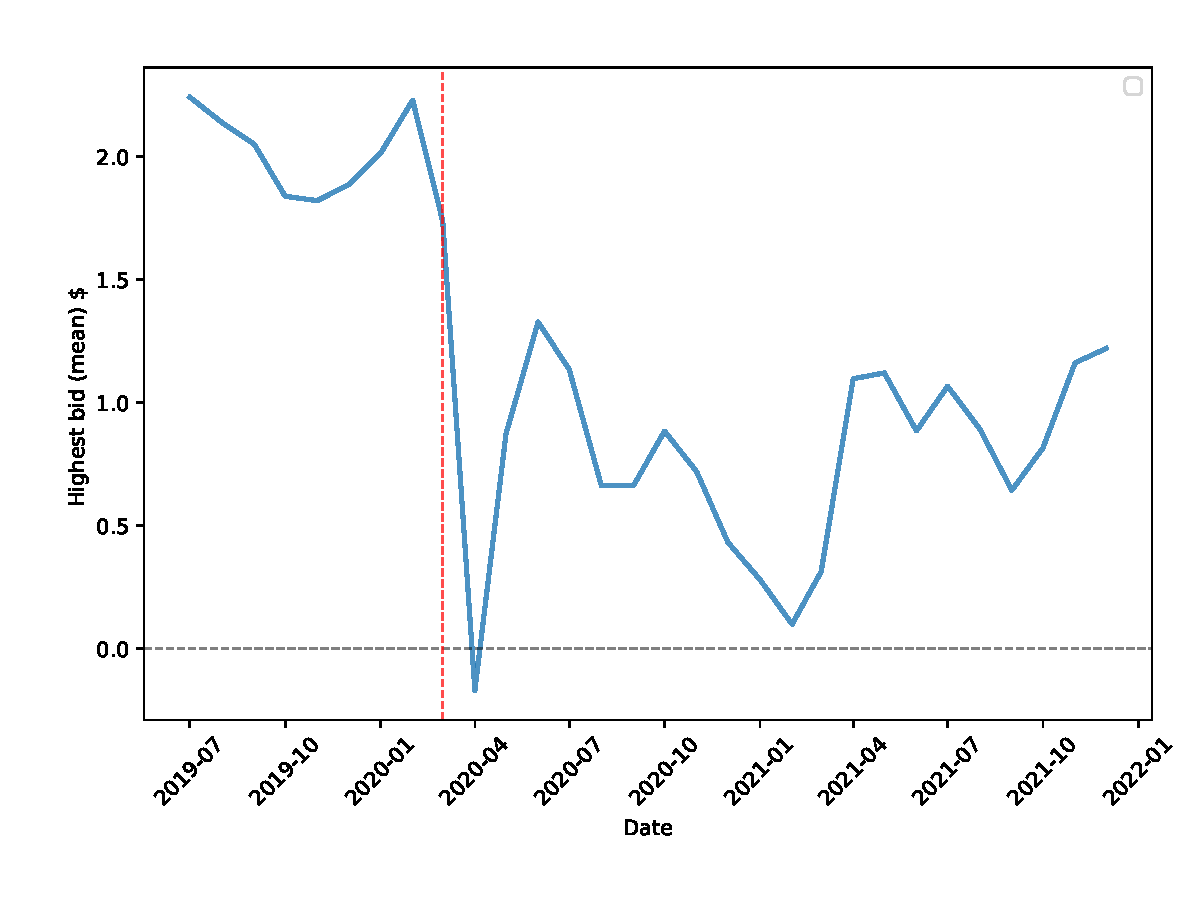
\includegraphics[width=0.998\textwidth]{../results/figures/w_winner_bid_mean_n_mat30_loan1_timeseries_nrmonthly_2.5_4_auction_netbid.pdf}
      \caption{ auction}
     \end{subfigure}
     \begin{subfigure}[b]{0.49\textwidth}
      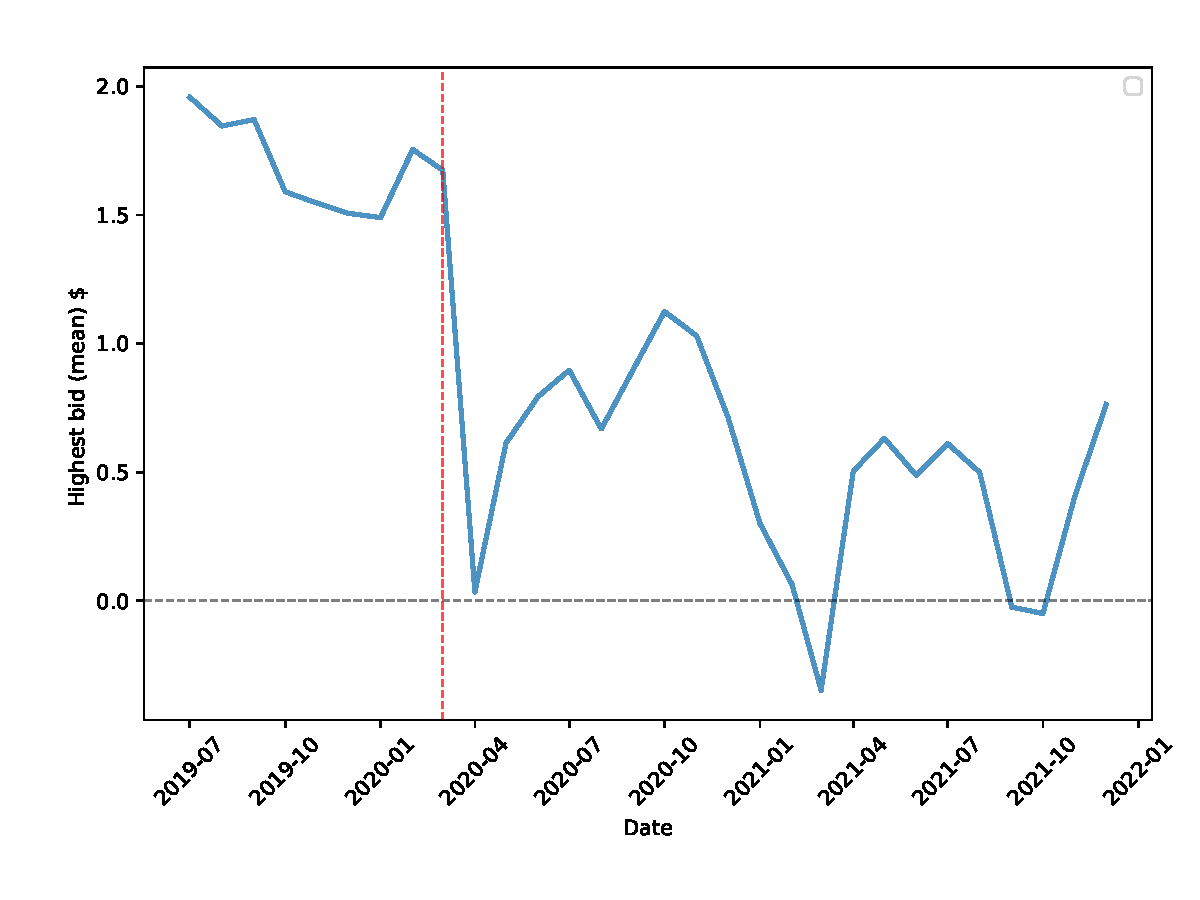
\includegraphics[width=0.998\textwidth]{../results/figures/w_winner_bid_mean_n_mat30_loan1_timeseries_nrmonthly_2.5_4_cash_window_netbid.pdf}
      \caption{cash window}
     \end{subfigure}
   \caption{Mean of highest net bid when investor buys (auction) and when GSE buys (cash window)} 
   \begin{minipage}{\textwidth}
      \footnotesize{\textit{Notes:} The figure shows the time series of auction outcomes for Conforming loans with a 30-year maturity.  The vertical line is March 1. The net bid is calculated by subtracting the TBA Bloomberg price for the same coupon and two forward months from the OB auction price. 
      The net bids are averaged accross coupons from 2.5 and 4.0 weighting by the loan amount. }
      \end{minipage}
\end{figure}



\begin{figure}[]
  \centering
     \begin{subfigure}[b]{0.49\textwidth}
      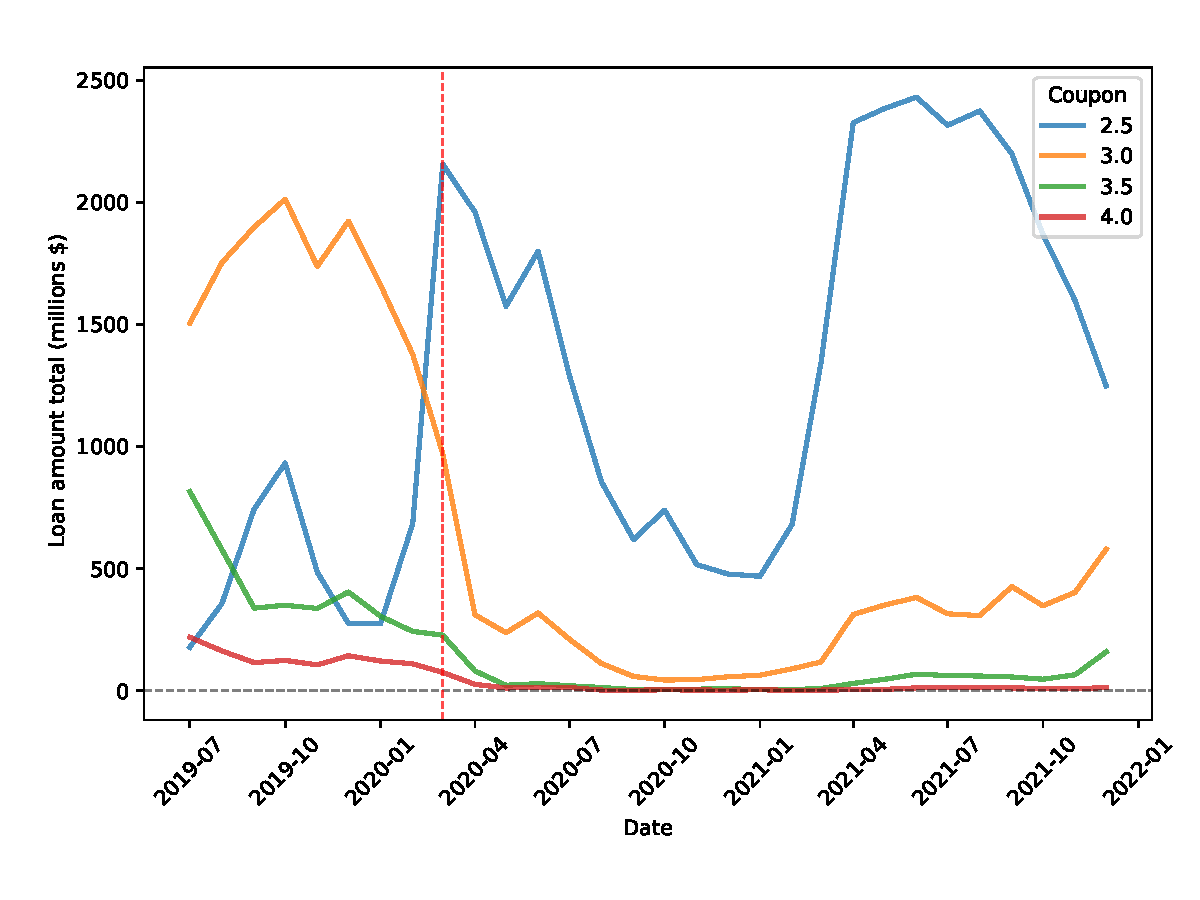
\includegraphics[width=0.998\textwidth]{../results/figures/LoanAmount_sum_mat30_loan1_timeseries_cpmonthly_2.5_4_auction.pdf}
      \caption{Loan amount auction}
     \end{subfigure}
      \begin{subfigure}[b]{0.49\textwidth}
        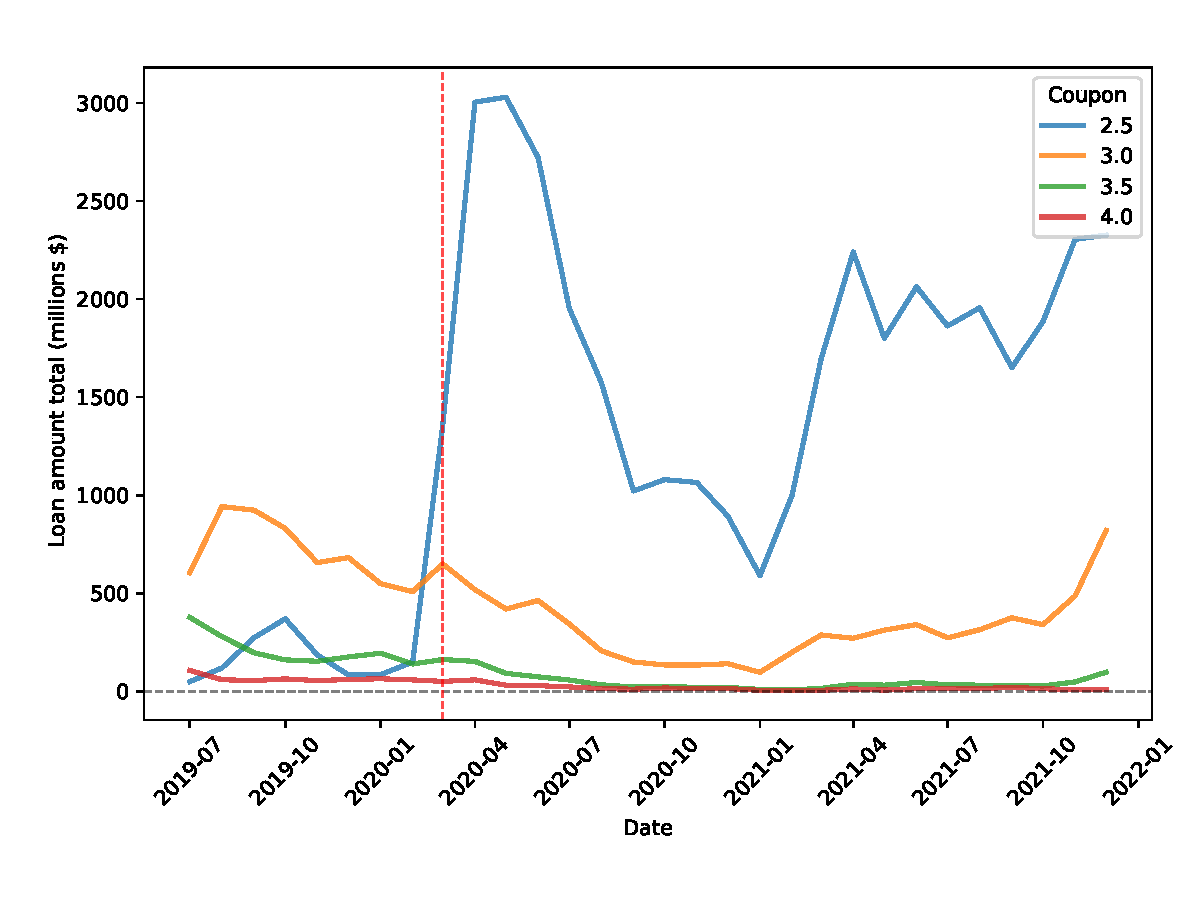
\includegraphics[width=0.998\textwidth]{../results/figures/LoanAmount_sum_mat30_loan1_timeseries_cpmonthly_2.5_4_cash_window.pdf}
        \caption{Loan amount cash window}
        \end{subfigure}
     \begin{subfigure}[b]{0.49\textwidth}
      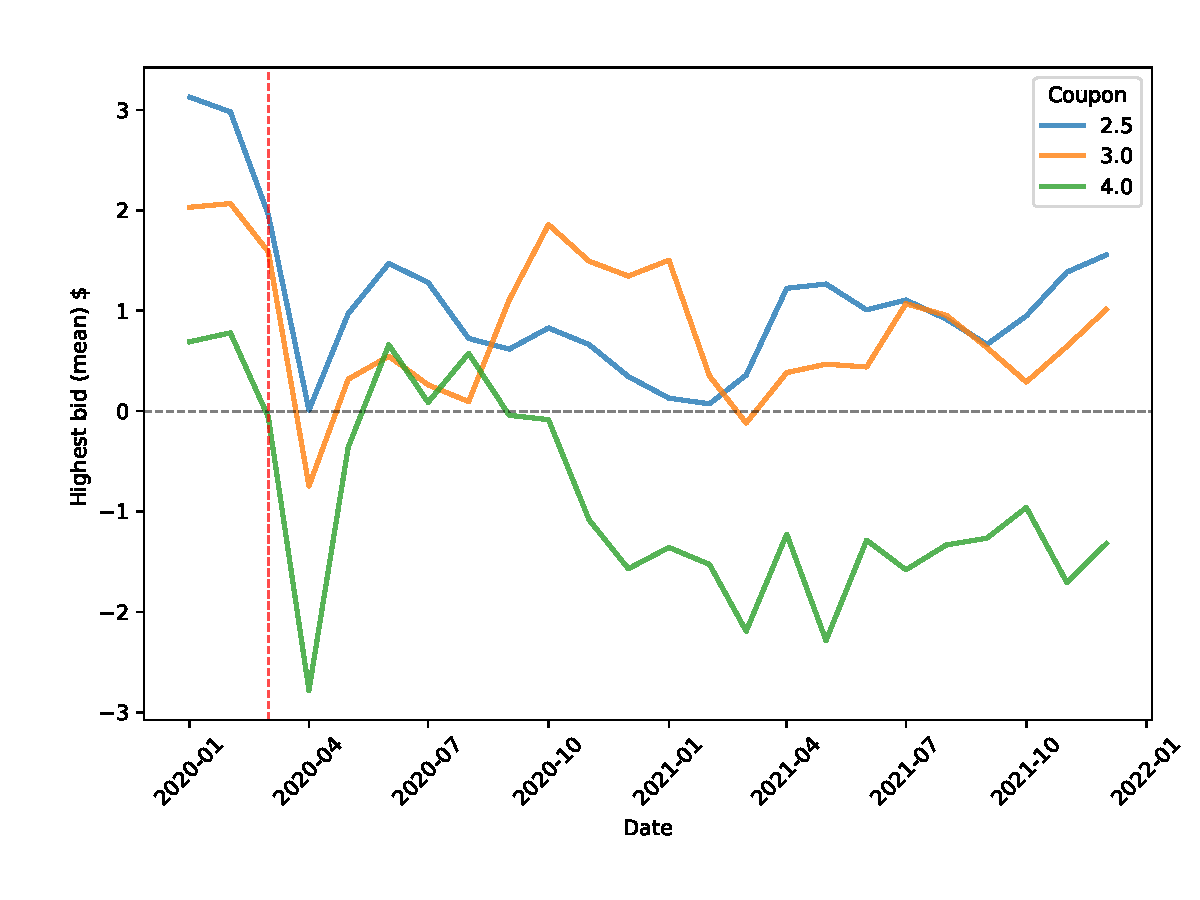
\includegraphics[width=0.998\textwidth]{../results/figures/winner_bid_mean_mat30_loan1_timeseries_cpmonthly_2.5_4_auction_netbid.pdf}
      \caption{ Mean of highest net bid auction}
     \end{subfigure}
     \begin{subfigure}[b]{0.49\textwidth}
      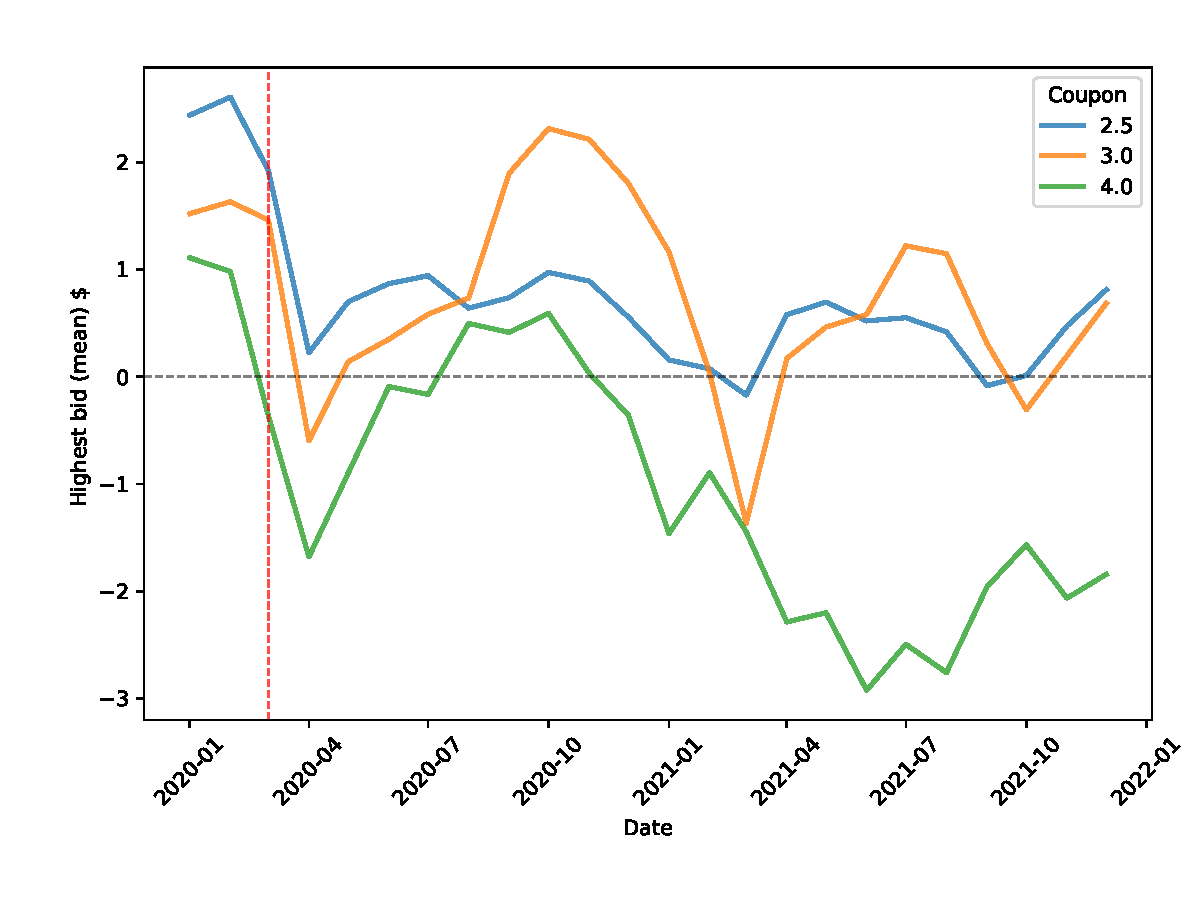
\includegraphics[width=0.998\textwidth]{../results/figures/winner_bid_mean_mat30_loan1_timeseries_cpmonthly_2.5_4_cash_window_netbid.pdf}
      \caption{ Mean of highest net bid cash window}
     \end{subfigure}
     \begin{subfigure}[b]{0.49\textwidth}
      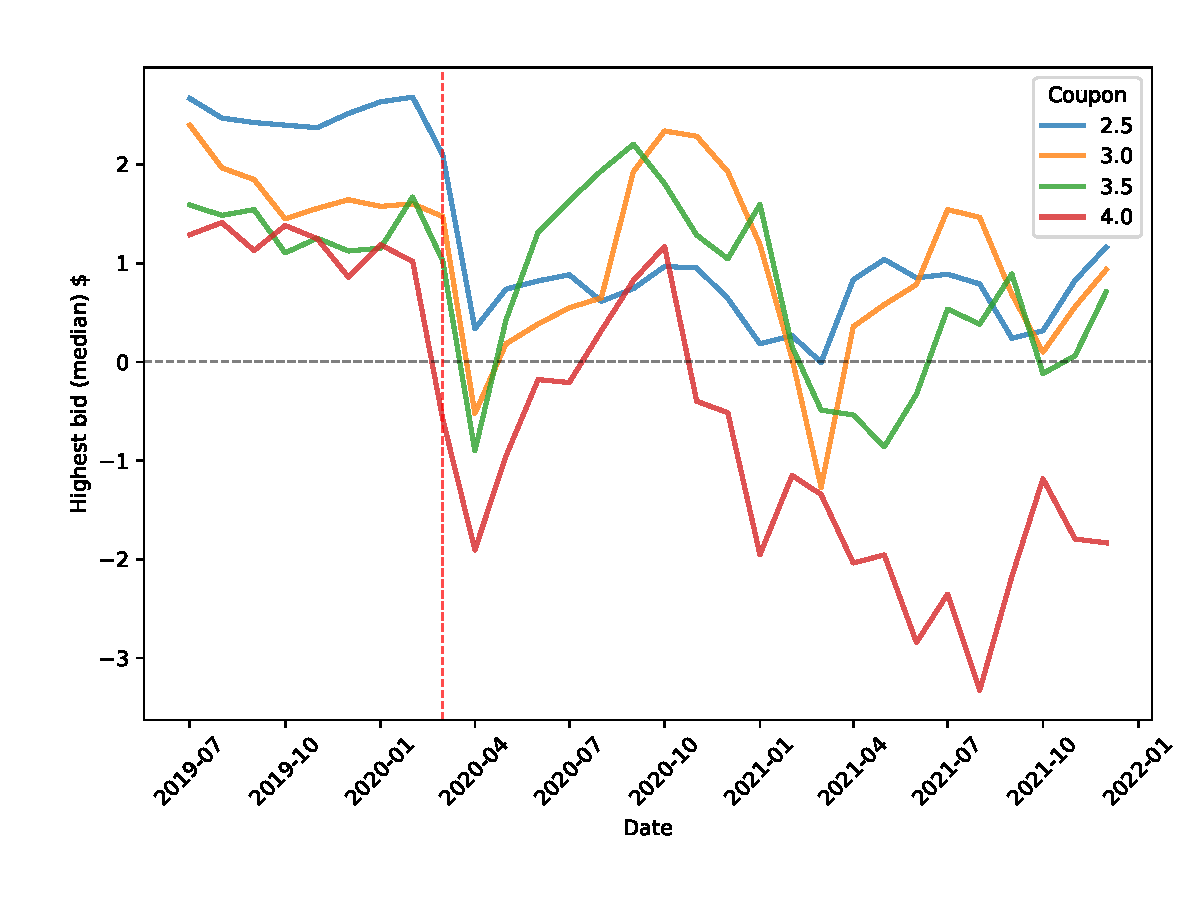
\includegraphics[width=0.998\textwidth]{../results/figures/winner_bid_median_mat30_loan1_timeseries_cpmonthly_2.5_4_cash_window_netbid.pdf}
      \caption{ Median of highest net bid auction}
     \end{subfigure}
     \begin{subfigure}[b]{0.49\textwidth}
      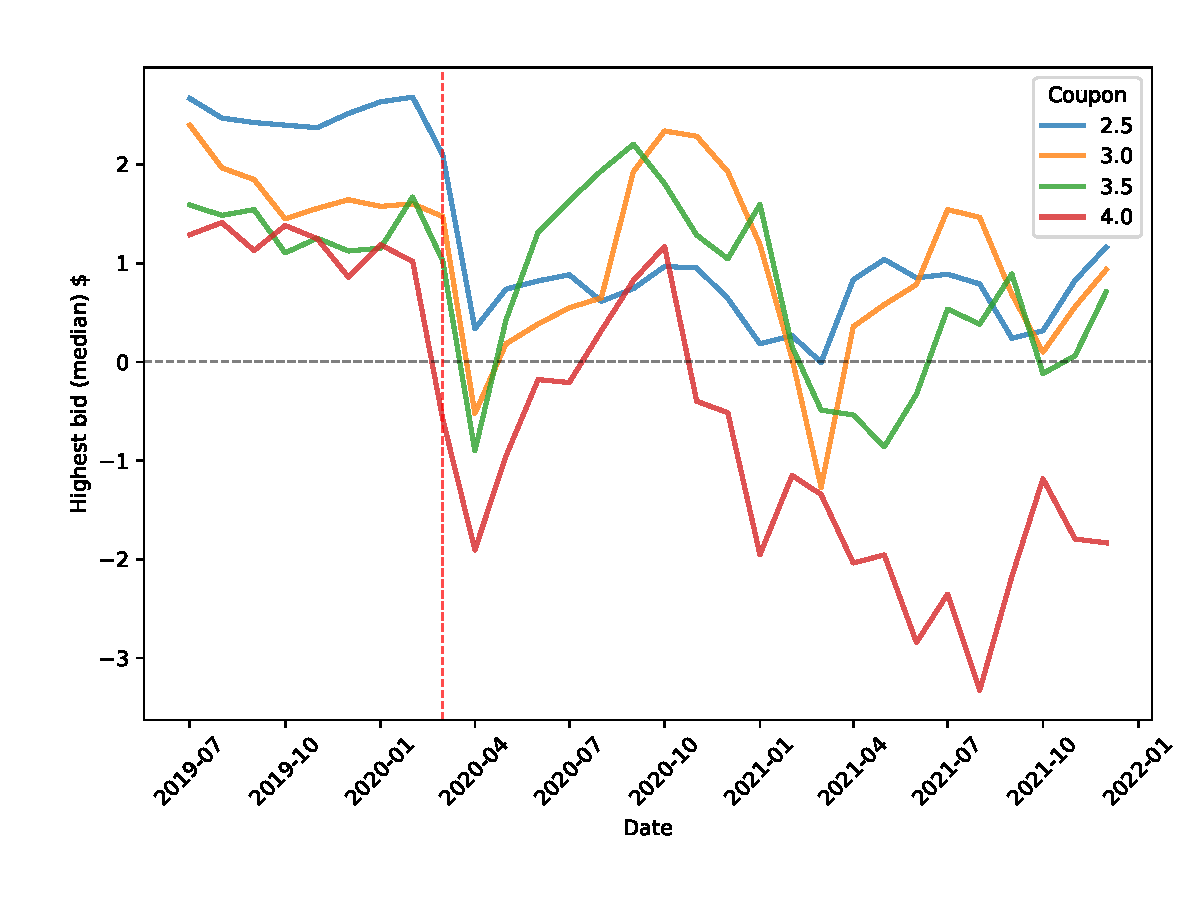
\includegraphics[width=0.998\textwidth]{../results/figures/winner_bid_median_mat30_loan1_timeseries_cpmonthly_2.5_4_cash_window_netbid.pdf}
      \caption{ Median of highest net cash window.}
     \end{subfigure}
      % \begin{subfigure}
      %   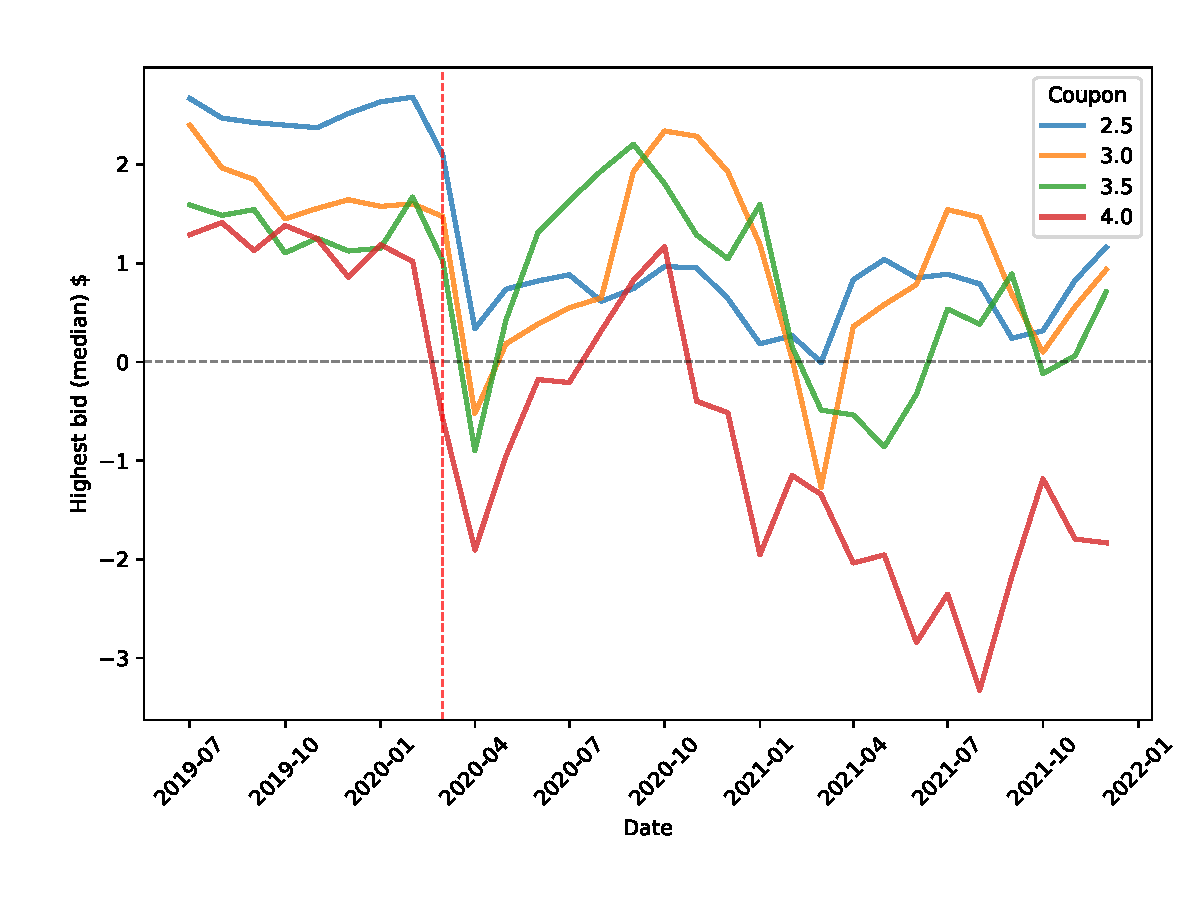
\includegraphics[width=0.998\textwidth]{../results/figures/winner_bid_median_mat30_loan1_timeseries_cpmonthly_2.5_4_cash_window_netbid.pdf}
      %   \caption{ Median of highest net bid cash window.}
      %   \end{subfigure}
   \caption{OB auction outcomes when investor buys (auction) and when GSE buys (cash window) by coupons. } 
   \begin{minipage}{\textwidth}
      \footnotesize{\textit{Notes:} The figure shows the time series of auction outcomes for Conforming loans with a 30-year maturity.  The vertical line is March 1. The net bid is calculated by subtracting the TBA Bloomberg price for the same coupon and two forward months from the OB auction price. }
      \end{minipage}
\end{figure}


\pagebreak
  \section{FED and Ob auction prices}

  In order to compare the FED and OB auction prices, we need to match the FED purchases with the OB auctions. We do this by matching coupon and trade date. We plot only Coupon 2.5 since it is the most traded coupon. The Bloomberg TBA price is one month forward.


\begin{figure}[h]
    \centering
    \begin{subfigure}[b]{0.49\textwidth}
      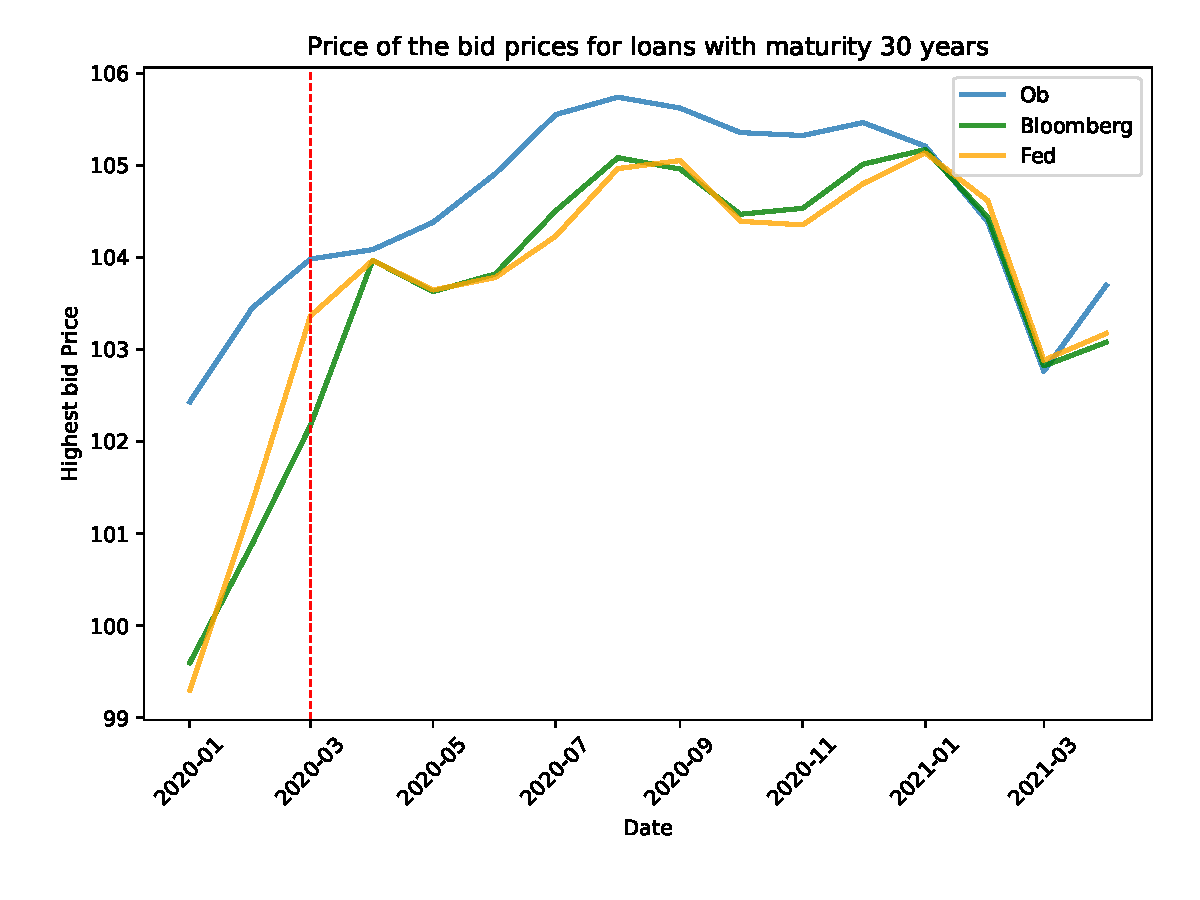
\includegraphics[width=0.998\textwidth]{../results/figures/fed_price_mean_mat30_loan1_timeseries_nrmonthly_2.5_4__fed_ob}
      \caption{Price date}
     \end{subfigure}
     \begin{subfigure}[b]{0.49\textwidth}
      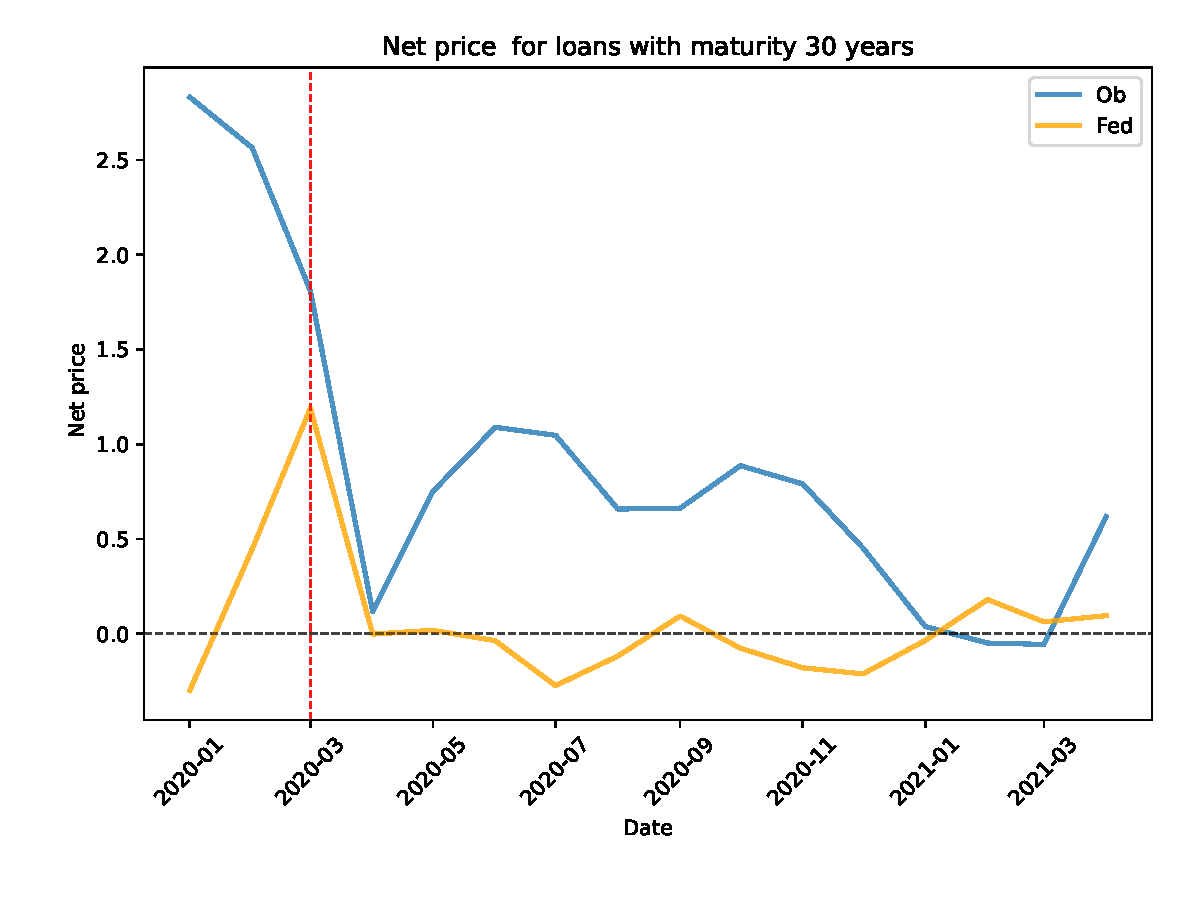
\includegraphics[width=0.998\textwidth]{../results/figures/fed_price_mean_mat30_loan1_timeseries_nrmonthly__normalized_fed_ob}
      \caption{Net price}
     \end{subfigure}
     \caption{Fed and OB auction prices for coupon 2.5 and 30-year maturity, TBA Bloomberg price is one month forward. } 
     \begin{minipage}{\textwidth}
      \footnotesize{\textit{Notes:} The figure shows the monthly time series of trade amounts and prices of FED  purchases of Fanny Mae and Fredy Mac products and 30-year maturity and Ob prices. Coupon selected is 2.5. } 
        \end{minipage}
\end{figure}





\end{document}
